\documentclass[a4paper,onecolumn]{extarticle}
\usepackage{geometry}
\usepackage[page,toc,titletoc,title]{appendix}
\usepackage{url}
\usepackage{caption}
\usepackage{subfigure}
\usepackage{subcaption}
\usepackage[sc]{mathpazo} % Use the Palatino font
\usepackage[T1]{fontenc} % Use 8-bit encoding that has 256 glyphs
\usepackage[utf8]{inputenc} % Use utf-8 as encoding
\linespread{1.05} % Line spacing - Palatino needs more space between lines
\usepackage{microtype} % Slightly tweak font spacing for aesthetics
\usepackage[spanish, activeacute]{babel}
 \decimalpoint
% \usepackage[hmarginratio=1:1,top=32mm,columnsep=20pt]{geometry} % Document marginshttps://www.overleaf.com/project/60211b96f72a79d4c7515e93
% \usepackage[hang, small,labelfont=bf,up,textfont=it,up]{caption} % Custom captions under/above floats in tables or figures
\usepackage{verbatim} % comentarios
\usepackage{listings}
\usepackage{xcolor}
\usepackage{wrapfig}
\lstset{
    inputencoding=utf8,
    frame=single,
    basicstyle=\fontsize{7}{10}\selectfont\ttfamily,
    basicstyle=\ttfamily\small,
    keywordstyle=\color{blue}\bfseries,
    identifierstyle=\color{black},
    commentstyle=\color{gray}\itshape,
    stringstyle=\color{red},
    numbers=left,
    numberstyle=\tiny\color{gray},
    stepnumber=1,
    numbersep=10pt,
    showspaces=false,
    showstringspaces=false,
    breaklines=true,
    breakindent=0pt,
    breakatwhitespace=false,
    tabsize=2,
    captionpos=b,
    literate={á}{{\'a}}1
        {ã}{{\~a}}1
        {é}{{\'e}}1
        {ó}{{\'o}}1
        {í}{{\'i}}1
        {ñ}{{\~n}}1
        {¡}{{!`}}1
        {¿}{{?`}}1
        {ú}{{\'u}}1
        {Í}{{\'I}}1
        {Ó}{{\'O}}1
}
\setlength{\parskip}{0.8em}
\usepackage{natbib}
\usepackage{enumitem}
% \setlist[itemize]{noitemsep} % Make itemize lists more compact
% \usepackage{abstract} % Allows abstract customization
% \renewcommand{\abstractnamefont}{\normalfont\bfseries} % Set the "Abstract" text to bold
% \renewcommand{\abstracttextfont}{\normalfont\small\itshape} % Set the abstract itself to small italic text
\usepackage{titlesec}

\usepackage{fancyhdr} % Headers and footers
\pagestyle{fancy} % All pages have headers and footers
\fancyhead{}
\lhead{Hugo Gómez Sabucedo}
\rhead{Minería de datos y modelización predictiva}

\renewcommand{\footrulewidth}{0.2pt}
\usepackage{titling} % Customizing the title section
\usepackage[breaklinks=true]{hyperref} % For hyperlinks in the PDF
%\usepackage{array}
%\newcolumntype{C}[1]{>{\centering\let\newline\\\arraybackslash\hspace{0pt}}m{#1}}
\usepackage{graphicx}
%\usepackage{lipsum} % NO NECESARIO LUEGO
%\usepackage{amsmath}
%\usepackage{wrapfig}
%\usepackage{multicol}
%\usepackage{bm}


\let\stdsection\section
\renewcommand\section{\newpage\stdsection}

%-------------------------------------------------------------------------------
%	TITLE SECTION
%-------------------------------------------------------------------------------

\setlength{\droptitle}{-4\baselineskip} % Move the title up



\title{\begin{center} \Huge Minería de datos y modelización predictiva \end{center}} % Article title
\author{
    \textsc{\Huge Hugo Gómez Sabucedo} \\ % Your name
    \large \href{mailto:hugogomezsabucedo@gmail.com}{hugogomezsabucedo@gmail.com} \\ [2ex] % Your email address
    \Large \textbf{Máster Big Data, Data Science \& Inteligencia Artificial} \\
    \normalsize Curso 2024-2025 \\
    \large Universidad Complutense de Madrid
}
\date{} % Leave empty to omit a date

\begin{document}
% Print the title
\maketitle
%\newpage
\tableofcontents
%\newpage
\begin{sloppypar}

%-------------------------------------------------------------------------
%	DOCUMENT
%-------------------------------------------------------------------------

\section{Introducción} \label{enunciado}
En esta práctica se nos pide, a partir de un archivo con datos sobre diferentes resultados electorales, seleccionar unas variables, con el objetivo
de construir tanto un modelo de regresión lineal, a partir de una variable objetivo continua; como un modelo de regresión logística, a partir de una
variable binaria. Para ello, se deberán asignar correctamente los tipos de los datos y realizar un análisis de los mismos, con el objetivo inicial 
de depurarlos, para asegurarnos que no tenemos variables incoherentes o que no se ajusten al modelo. A continuación, se corregirán los errores que se 
hayan detectado, así como los valores atípicos y perdidos. Una vez con los datos limpios, podremos analizar las relaciones entre las distintas variables 
input y las variables objetivo, para poder proceder con la creación de los dos modelos solicitados, para cada una de las variables.

Cada registro del archivo viene identificado por Name y CodigoProvincia (ya que, observando el conjunto de datos, se han encontrado municipios con el mismo
nombre pero en provincias diferentes). Adicionalmente, contienen información sobre la CCAA a la que pertenecen. Por otra parte, tenemos las variables objetivo,
que se dividen en las variables continuas (AbstentionPtge, el porcentaje de abstención; IzdaPct, el porcentaje de votos a partidos de izquierdas; DchaPct, el
porcentaje de votos a partidos de derechas; y OtrosPct, el porcentaje de votos a otros partidos); y las variables binarias o dicotómicas (AbstencionAlta, que 
vale 1 si el porcentaje de abstención es mayor al 30\% o 0 en otro caso; Izquierda, que toma valor 1 si la suma de votos a los partidos de izquierda es 
superior a la suma de votos a derchas y otros, y 0 en caso contrario; y Derecha, análoga a la anterior, pero para partidos de derechas). De estas, se
escogerá \textbf{AbstentionPtge} para realizar la regresión lineal; e \textbf{Izquierda} para realizar la regresión logística.

Por otra parte, tenemos un conjunto de 29 variables explicativas, las cuales no entraremos a explicar en detalle, pero que se corresponden con aspectos 
demográficos o sociológicos de los distintos municipios, como puede ser el porcentaje de población por tramos de edad, el porcentaje de desempleo por edades 
o sectores, el número de empresas de los municipios por tipo de actividad y la actividad principal del mismo, el porcentaje de población respecto a su CCAA 
y provincia de nacimiento, o, evidentemente, el censo, población, superficie y densidad del municipio.

De esta forma, nuestro objetivo será construir un modelo de regresión lineal para la variable AbstentionPtge y un modelo de regresión logística para la 
variable Izquierda, que nos permitan en el primer caso predecir el porcentaje de abstención, y en el segundo caso, la probabilidad de que los partidos de 
izquierdas sean los más votados.

\section{Importación de datos y análisis descriptivo}\label{importacionAnalisis}
\subsection{Importación}\label{importacion}
Para importar los datos, una vez establecido el directorio de trabajo a la carpeta correspondiente con \texttt{os.chdir}, se emplea la siguiente instrucción:
\begin{lstlisting}[language=Python, numbers=none]
    datos = pd.read_excel("DatosElecciones.xlsx", sheet_name='DatosEleccionesEspaña')
\end{lstlisting}

Lo primero que haremos será definir el ID de los datos, que es el nombre del ayuntamiento y el código de la provincia, mediante la instrucción:
\begin{lstlisting}[language=Python,numbers=none]
datos.set_index(["Name", "CodigoProvincia"], inplace=True, drop=True)
\end{lstlisting}

Mediante \texttt{datos.head(5)} podemos ver las 5 primeras filas, y con \texttt{datos.dtypes} podemos ver los tipos de datos de las variables, lo que 
usaremos para comprobar que cada una de las variables tiene asignado el tipo que le corresponde (es decir, numérica o categórica). Se observa que únicamente
se han importado como categóricas (tipo \texttt{Object}) las variables Name, CCAA, ActividadPpal y Densidad, mientras que el resto se han importado bien 
como int o bien como float. Debemos, por tanto, transformar a categóricas las tres variables objetivo binarias: Izquierda, Derecha y AbstencionAlta, mediante 
la función \texttt{astype(str)}. A continuación, crearemos una lista con todas las variables, y las dividiremos en numéricas y categóricas.
\begin{lstlisting}[language=Python]
    numsACategoricas = ['Izquierda', 'Derecha', 'AbstencionAlta']
    for v in numsACategoricas:
        datos[v] = datos[v].astype(str)

    variables = list(datos.columns)
    
    numericas = datos.select_dtypes(include=['int', 'int32', 'int64','float', 'float32', 'float64']).columns
    categoricas = [v for v in variables if v not in numericas]
\end{lstlisting}

\begin{lstlisting}[numbers=none]
    Izquierda         int64
    Derecha           int64
    AbstencionAlta    int64
\end{lstlisting}

Podemos hacer de nuevo un print de `categoricas` para comprobar que las variables están asignadas correctamente: 
\begin{lstlisting}[numbers=none]
    ['Name', 'CCAA', 'AbstencionAlta', 'Izquierda', 'Derecha', 'ActividadPpal', 'Densidad']
\end{lstlisting}

Puesto que todas las variables están ya correctamente asignadas, podemos pasar directamente al análisis descriptivo de las mismas.

\subsection{Análisis descriptivo}\label{analisis}
\begin{wrapfigure}[11]{l}{4.75cm}
    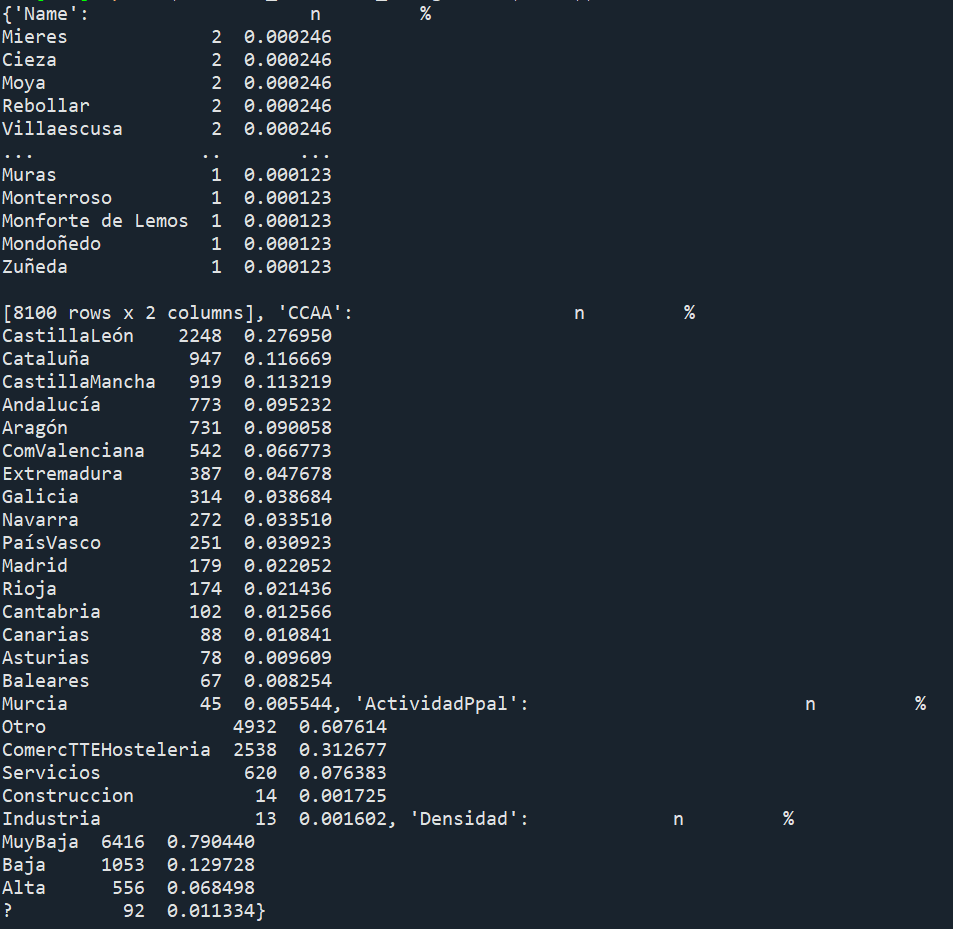
\includegraphics[width=4.5cm]{ejecuciones/analizar_categoricas.png}
\end{wrapfigure}

A continuación haremos el análisis descriptivos de las variables explicativas, comenzando en primer lugar por las categóricas.

Como podemos ver, hay algunos municipios que se repiten dos veces, pero esto es debido a que existe el mismo municipio en dos provincias (por ejemplo, Mieres 
en Asturias, y Mieres (o Mieras) en Girona). Por otra parte, en la variable CCAA, tenemos múltiples comunidades con una frecuencia inferior al 5\%, que se 
considera que están poco representadas. Tendremos que reagruparlas en el apartado \ref{errores}. Una situación similar nos encontramos con ActividadPal,
donde las categorías Construcción e Industria tienen una frecuencia de 0.001 ambas. Las reagruparemos con otra categoría. Respecto a Densidad, la única categoría 
poco representada es \textit{?}, que nos puede indicar que se trataría de valores perdidos.

Analizamos también los valores únicos de cada una de las variables, mediante el siguiente código, y vemos que los valores de las CCAA y la ActividadPpal son los
correctos y los esperados, que las variables Izquierda, Derecha y AbstencionAlta solo toman valores 1 y 0, y confirmamos el caso anterior de que la variable 
Densidad tiene valores perdidos.
\begin{lstlisting}[language=Python,numbers=none]
for cat in categoricas:
    print(datos[cat].unique())
\end{lstlisting}
\begin{lstlisting}[numbers=none]
['Abadía' 'Abertura' 'Acebo' ... 'Zarzosa de Río Pisuerga' 'Zazuar'
'Zuñeda']
['Extremadura' 'Andalucía' 'ComValenciana' 'CastillaMancha' 'Galicia'
'Cataluña' 'PaísVasco' 'Aragón' 'CastillaLeón' 'Rioja' 'Madrid' 'Murcia'
'Navarra' 'Asturias' 'Canarias' 'Cantabria' 'Baleares']
['0' '1']
['1' '0']
['0' '1']
['Otro' 'ComercTTEHosteleria' 'Servicios' 'Construccion' 'Industria']
['MuyBaja' '?' 'Baja' 'Alta']
\end{lstlisting}

Analizamos ahora las variables numéricas. En primer lugar, analizamos los valores distintos con \texttt{cuentaDistintos}, donde vemos que todas las variables 
tienen un número suficiente de datos. La que menos valores distintos tiene es PersonasInmueble con 282 valores, pero es un valor esperable. Empleamos 
la función \texttt{describe} para hallar valores como la media o los cuartiles, ampliándola con la asimetría, la curtosis y el rango.
\begin{lstlisting}[language=Python]
descriptivos_num = datos.describe().T
for num in numericas:
    descriptivos_num.loc[num, "Asimetria"] = datos[num].skew()
    descriptivos_num.loc[num, "Kurtosis"] = datos[num].kurtosis()
    descriptivos_num.loc[num, "Rango"] = np.ptp(datos[num].dropna().values)
\end{lstlisting}

Podemos ver que las variables Poblacion, TotalCensus, inmuebles, Pob2010 y totalEmpresas presentan un rango muy elevado, lo cual tiene sentido debido a
ciudades como Madrid o Barcelona tienen una población muy elevada, lo cual impacta en las otras cuatro variables mencionadas. Podríamos pensar en aplicar 
alguna transformación, por ejemplo logarítmica, para reducir el impacto de estas anomalías, pero he considerado que estos aportan un valor, ya que estos 
municipios con población elevada deberían de alguna forma poder tener más peso. Por otra parte, se observan algunas variables que, siendo porcentajes, bien 
tienen valores mínimos negativos, como Age\_over65\_pct y ForeignersPtge, bien tienen valores máximos mayores que 100, comoAge\_19\_65\_pct o SameComAutonPtge. 
Este caso de porcentajes negativos o mayores que 100 se encuentra también para PobChange\_pct, pero aquí sí que tiene sentido, ya que pueden indicar o un 
decrecimiento de la población o un aumento muy grande de la misma. Por último, se ve que el valor máximo de Explotaciones es de 99999, lo cual nos podría 
indicar que esta variable tiene algún valor perdido.

\begin{wrapfigure}[13]{L}{8cm}
    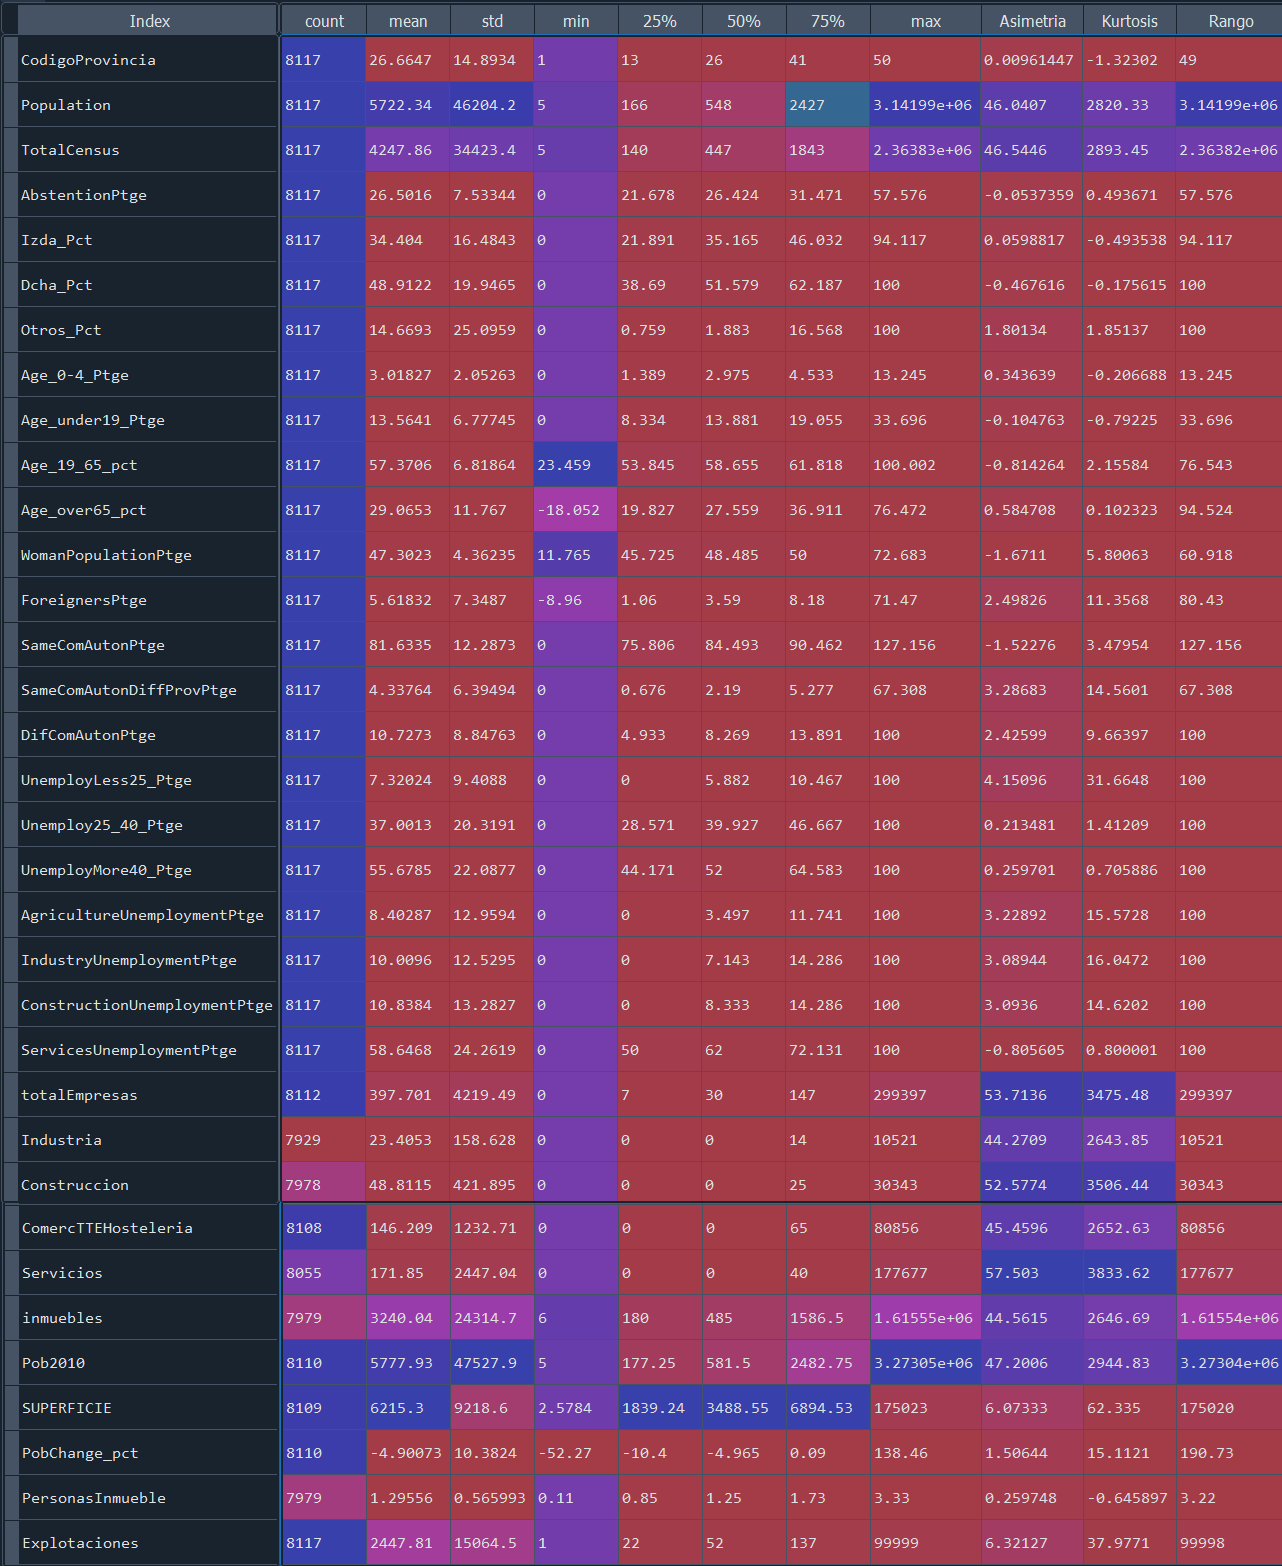
\includegraphics[width=8cm]{ejecuciones/descriptivos.png}
    \small{\caption{Análisis descriptivo de variables numéricas}}
\end{wrapfigure} 

Por otra parte, analizamos también los valores faltantes, y nos encontramos que las siguientes variables presentan algún valor faltante, pero en ningún caso 
un número tan elevado como para que nos podamos plantear descartarlas.
\begin{lstlisting}[numbers=none]
totalEmpresas            5
Industria              188
Construccion           139
ComercTTEHosteleria      9
Servicios               62
inmuebles              138
Pob2010                  7
SUPERFICIE               8
PobChange_pct            7
PersonasInmueble       138
\end{lstlisting}

Una vez hemos analizado todos los datos y detectado todos los errores posibles (seguramente haya más, pero evidentemente es imposible detectar todos los 
errores que presentan los datos), podremos pasar a corregirlos.
\\
\section{Corrección de errores}\label{errores}
En relación a las variables categóricas, como vimos en el apartado \hyperref[analisis]{anterior}, únicamente debemos realizar reagrupaciones. Por una parte,
reagruparemos las categorías Construccion e Industria de la variable \textit{ActividadPpal}, en la categoría Otro, debido a las bajas frecuencias observadas 
para estas categorías. Esto se hace mediante el siguiente código:
\begin{lstlisting}[language=Python,numbers=none]
datos['ActividadPpal'] = datos['ActividadPpal'].replace(\{'Construccion': 'Otro', 'Industria': 'Otro'\})
\end{lstlisting}

Respecto a la variable \textit{CCAA}, no podemos agrupar aleatoriamente, sino que debemos hacerlo teniendo en cuenta aquellas que presenten características 
similares. En este caso ya que estudiaremos la variable AbstentionPtge, hemos decidido tener este parámetro en cuenta para realizar la agrupación, obteniendo 
los resultados que se ven en la figura \ref{fig:CCAAbypct}.
\begin{lstlisting}[language=Python,numbers=none]
promedio_abstencion = datos.groupby('CCAA')['AbstentionPtge'].mean().reset_index()
\end{lstlisting}

Las agrupaciones que realizaremos serán entonces: Canarias, Asturias, Baleares y País Vasco; Galicia y Navarra; Murcia, Cantabria y Extremadura; Madrid y Aragón; 
y Rioja y la Comunidad Valenciana. Si ahora volvemos a analizar la frecuencia de los valores para la variable, vemos en la figura \ref{fig:CCAAreagrupada} que 
la nueva ''CCAA'' con menos frecuencia es la agrupación de Canarias, Asturias, Baleares y País Vasco, con un $5.96\%$.

\begin{figure}[h!]
    \centering
    \begin{minipage}{0.35\textwidth}
        \centering
        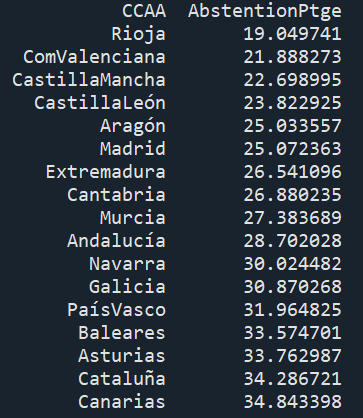
\includegraphics[width=0.75\textwidth]{ejecuciones/CCAA_porabst.png}
        \caption{Abstención promedio por CCAA}
        \label{fig:CCAAbypct}
    \end{minipage}%
    \hspace{0.05\textwidth} % Espacio entre las imágenes
    \begin{minipage}{0.35\textwidth}
        \centering
        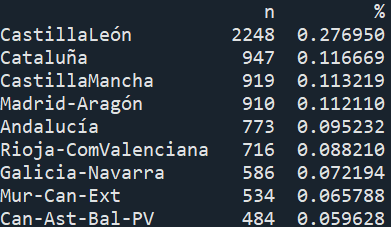
\includegraphics[width=\textwidth]{ejecuciones/CCAA_reagrupadas.png}
        \caption{CCAA tras reagrupación}
        \label{fig:CCAAreagrupada}
    \end{minipage}
\end{figure}

Lo siguiente que haremos será sustituir los valores que encontramos como perdidos (el 99999 que encontramos en Explotaciones), así como algún posible NaN que
pueda haber en los datos y que no hayamos detectado.
\begin{lstlisting}[language=Python]
for v in categoricas:
    datos[v] = datos[v].replace('nan', np.nan)
    
datos['Explotaciones'] = datos['Explotaciones'].replace(99999,np.nan)
\end{lstlisting}

Por último, corregiremos los errores que encontramos con los porcentajes, indicando que se pasen a valores perdidos aquellos donde el porcentaje no esté
entre 0 y 100.
\begin{lstlisting}[language=Python]
datos['Age_over65_pct'] = [x if 0<=x<=100 else np.nan for x in datos['Age_over65_pct']]
datos['ForeignersPtge'] = [x if 0<=x<=100 else np.nan for x in datos['ForeignersPtge']]
datos['Age_19_65_pct'] = [x if 0<=x<=100 else np.nan for x in datos['Age_19_65_pct']]
datos['SameComAutonPtge'] = [x if 0<=x<=100 else np.nan for x in datos['SameComAutonPtge']]
\end{lstlisting}

Una vez hecho esto, definimos las variables objetivo \texttt{varObjCont = datos[`AbstentionPtge`]} y \texttt{varObjBin = datos[`Izquierda`]}, y eliminamos
todas las variables objetivo de los datos, mediante la funcion \texttt{.drop} . A partir de esto, renombramos los datos como datos\_input, y creamos las 
variables numericas\_input y categoricas\_input con la división en categóricas y numéricas de las variables.

\section{Análisis de valores atípicos}\label{atipicos}
Para tratar los valores atípicos, en primer lugar, mediremos la proporción de valores missing que hay por cada variable, y tratándolos con la función 
\texttt{atipicosAmissing}, empleando para ello el código:
\begin{lstlisting}[language=Python]
resultados = {x: atipicosAmissing(datos_input[x])[1] / len(datos_input) for x in numericas_input}
for x in numericas_input:
    datos_input[x] = atipicosAmissing(datos_input[x])[0]
\end{lstlisting}
Así, nos encontramos con los siguientes porcentajes de valores atípicos que, como podemos observar, se encuentran preesentes en la mayoría de variables. Cabe 
destacar el elevado número de valores atípicos en, por ejemplo, Population o TotalCensus que, como comentamos en el \ref{analisis}, se debe a ciudades con 
mucha población, y que en este caso serán tratados como atípicos y, por tanto, convertidos a missing. Otra opción podría haber sido hacer una transformación 
logarítmica de los datos, pero se observó que, aun realizándola, se seguían detectando numerosos valores atípicos, por lo que lo más adecuado parece ser 
dejar que sean tratados directamente como atípicos.
\begin{lstlisting}[numbers=none]
{'Population': 0.05297523715658495, 'TotalCensus': 0.050880867315510656, 'Age_0-4_Ptge': 0.0, 'Age_under19_Ptge': 0.0, 'Age_19_65_pct': 0.00012319822594554638, 'Age_over65_pct': 0.0, 'WomanPopulationPtge': 0.0, 'ForeignersPtge': 0.006036713071331773, 'SameComAutonPtge': 0.00012319822594554638, 'SameComAutonDiffProvPtge': 0.0024639645189109276, 'DifComAutonPtge': 0.00012319822594554638, 'UnemployLess25_Ptge': 0.0, 'Unemploy25_40_Ptge': 0.0, 'UnemployMore40_Ptge': 0.0, 'AgricultureUnemploymentPtge': 0.0013551804854010103, 'IndustryUnemploymentPtge': 0.0, 'ConstructionUnemploymentPtge': 0.0, 'ServicesUnemploymentPtge': 0.0, 'totalEmpresas': 0.10484169027965998, 'Industria': 0.09239866945915978, 'Construccion': 0.0903042996180855, 'ComercTTEHosteleria': 0.09868177898238266, 'Servicios': 0.11851669335961562, 'inmuebles': 0.09042749784403105, 'Pob2010': 0.0974497967229272, 'SUPERFICIE': 0.027103609708020206, 'PobChange_pct': 0.0012319822594554638, 'PersonasInmueble': 0.0, 'Explotaciones': 0.050880867315510656}
\end{lstlisting}

\section{Análisis de valores perdidos}\label{perdidos}
En el caso de los valores perdidos, lo primero que haremos será obtener la matriz de correlación de valores ausentes, mediante la función proporcionada 
\texttt{patron\_perdidos}, a la que se realizó una modificación para eliminar los valores numéricos de la misma.
\begin{figure}[h!]
    \centering
    \begin{minipage}{0.50\textwidth}
        \centering
        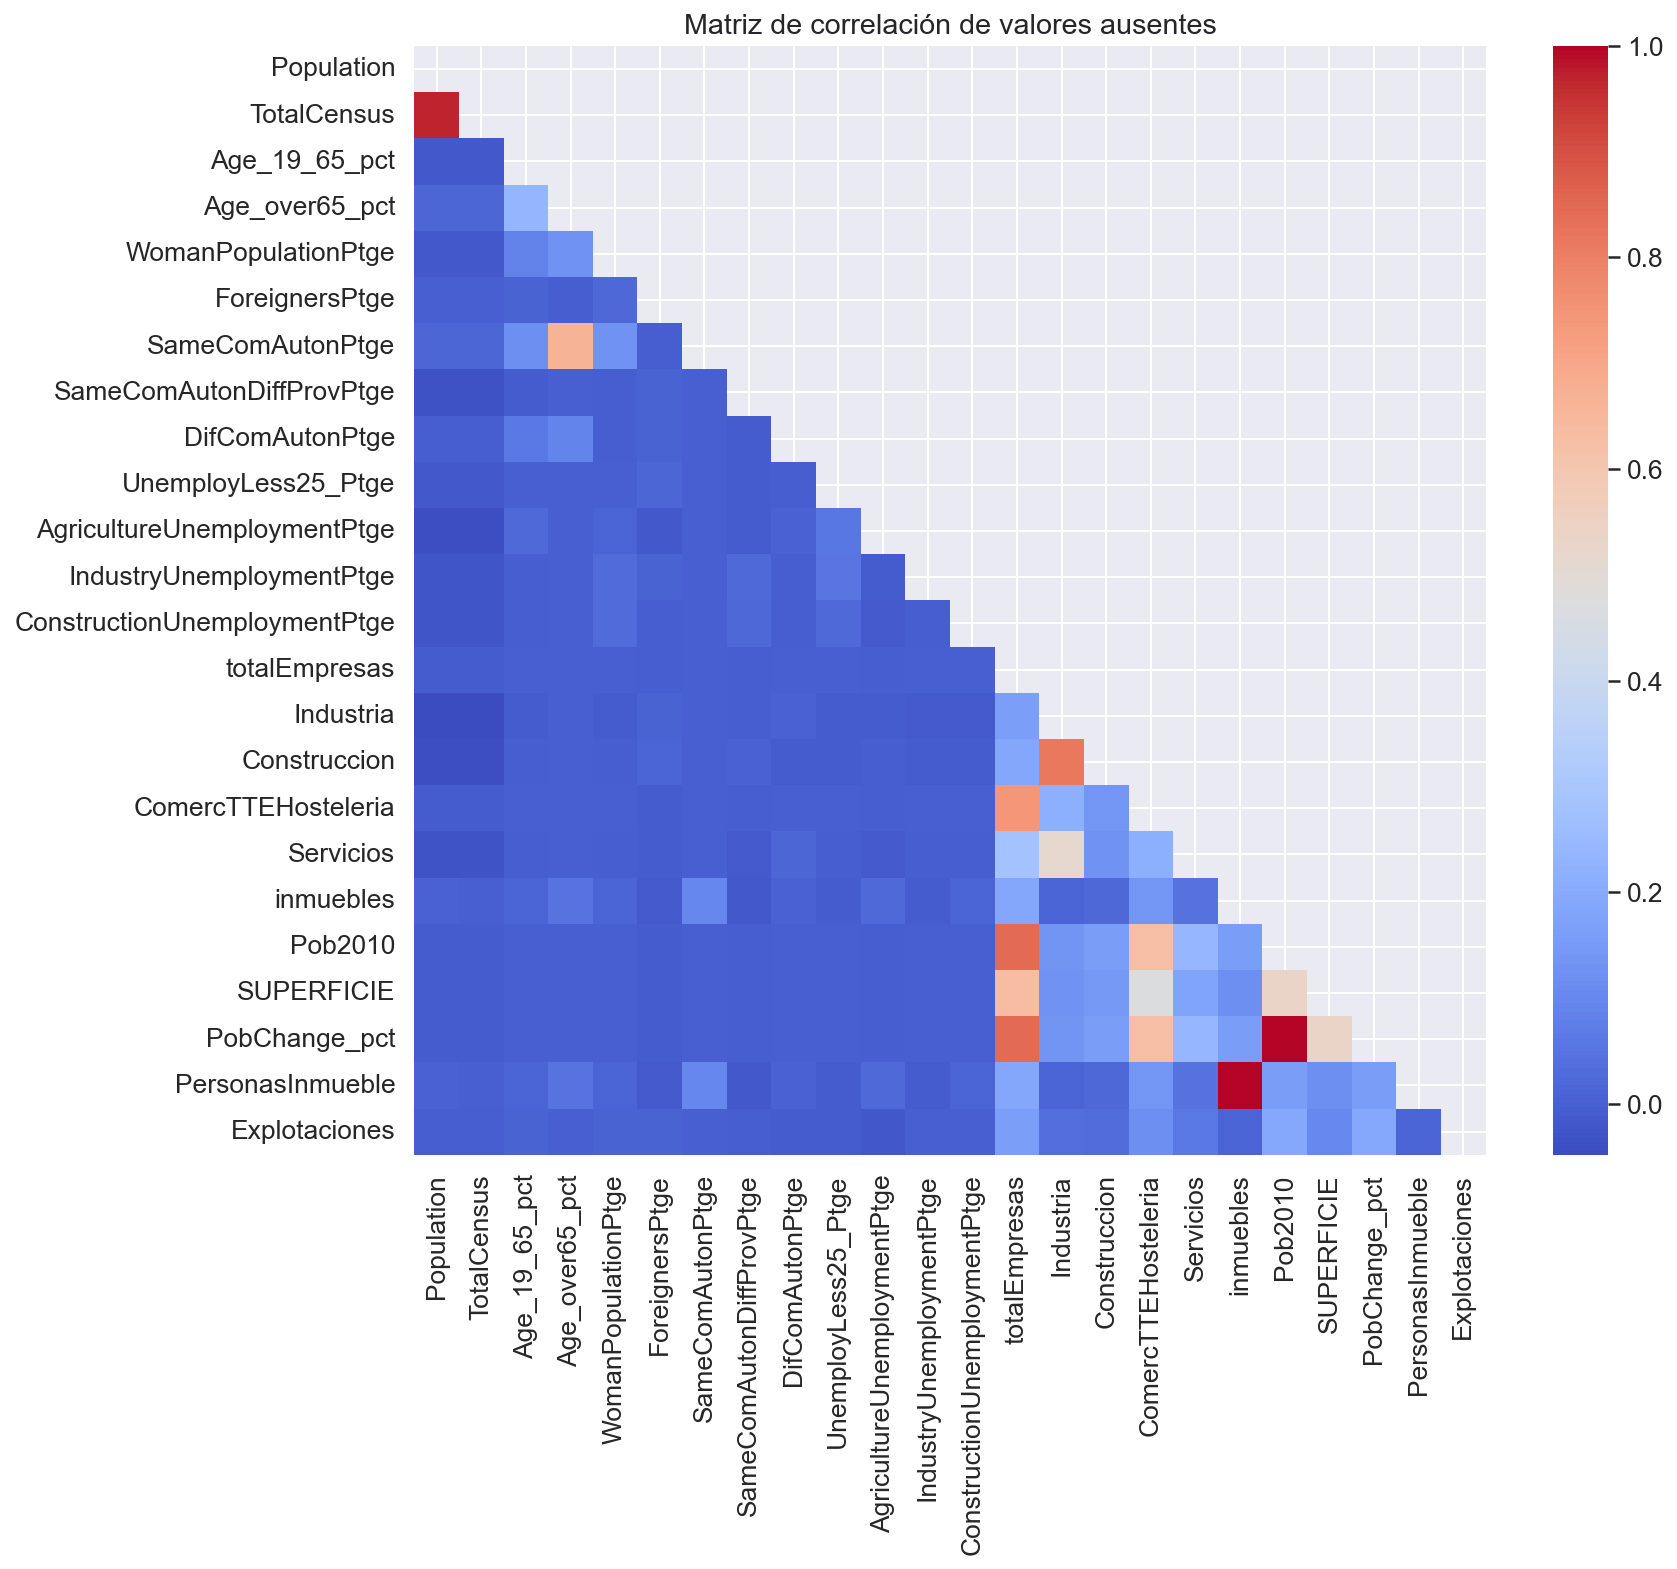
\includegraphics[width=\textwidth]{ejecuciones/perdidos.png}
        \caption{Matriz de valores perdidos}
        \label{fig:perdidos}
    \end{minipage}%
    \hspace{0.05\textwidth} % Espacio entre las imágenes
    \begin{minipage}{0.40\textwidth}
        \centering
        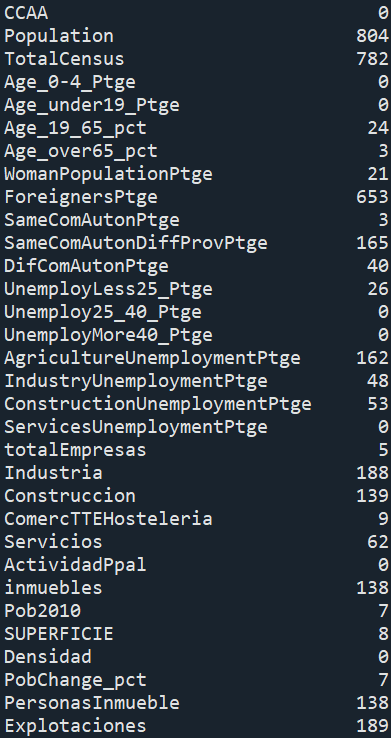
\includegraphics[width=0.5\textwidth]{ejecuciones/perdidos_porvar.png}
        \caption{Valores perdidos por variable}
        \label{fig:perdidosporvar}
    \end{minipage}
\end{figure}

Como podemos ver, se observa una gran correlación entre TotalCensus y Población, Inmuebles y PersonasInmueble y Pob2010 y PobChange\_pct. Esto puede tener sentido,
ya que son variables que están relacionadas entre si. También se observa un gran número de valores perdidos en ForeignersPtge, concretamente 653, aunque esto 
podría tener explicación en algunos municipios que no tengan ninguna persona extranjera censada. Se observa también un número elevado de valores perdidos en las 
variables AgricultureUnemploymentPtge, SameComAutonDiffProvPtge, Industria, Construccion o Explotaciones, todos los cuales tendremos que tratar posteriormente. 
Sin embargo, si analizamos la proporción de valores missing por variable (prop\_missingsVars), vemos que las que más valores perdidos tienen son, naturalmente, 
Population y TotalCensus, con un 9.905\% y un 9.634\% respectivamente, seguidas de ForeignersPtge con un 8.044\% y luego las otras variables comentadas, con 
apenas un 2\%. Ninguna supera, por tanto, el 50\% de valores missing con los que se eliminaría la variable.

\begin{lstlisting}[language=Python]
datos_input[variables_input].isna().sum()
prop_missingsVars = datos_input.isna().sum()/len(datos_input)

#Media de valores perdidos para cada una de las filas
datos_input['prop_missings'] = datos_input.isna().mean(axis = 1)
datos_input['prop_missings'].describe()
len(datos_input['prop_missings'].unique())

# Transformamos a categorica
datos_input["prop_missings"] = datos_input["prop_missings"].astype(str)
variables_input.append('prop_missings')
categoricas_input.append('prop_missings')
\end{lstlisting}

Por otra parte, se crea la columna \textit{prop\_missings}, que representa el porcentaje de valores perdidos por cada una de las filas. Si hacemos un describe 
de esta variable, vemos que la que más valores perdidos tiene presenta un 33.33\% de valores perdidos, mientras que la mediana es apenas un 3.03\%. Ya que 
ninguno de los registros no tiene tampoco más de un 50\% de datos faltantes, vemos que no es necesario eliminar ninguno. Lo que si realizaremos es un análisis 
de los valores únicos de esta nueva columna creada, ya que se crea como continua, pero podría tener sentido que fuese categórica. Y, efectivamente, vemos que 
tiene solamente 9 valores únicos, por lo que, como se indica, se transforma a categórica esta variable.

Una vez ya hemos analizado los valores missing, tenemos que ver como vamos a tratarlos. Para ello, se nos proporcionan dos funciones en el script de clase,
\texttt{ImputacionCuant} e \texttt{ImputacionCuali}. Por ello, solamente tendremos que aplicarlas a las variables, por una parte a las variables numéricas, 
y por otra parte a las variables categóricas.
\begin{lstlisting}[language=Python]
for x in numericas_input:
    datos_input[x] = ImputacionCuant(datos_input[x], 'aleatorio')
    
for x in categoricas_input:
    datos_input[x] = ImputacionCuali(datos_input[x], 'aleatorio')
\end{lstlisting}

Lo último que nos queda por hacer es revisar, con \texttt{\textbf{datos\_input.isna().sum()}}, que no quede ningún valor faltante. Aunque no se incluya aquí 
la salida de este comando, se comprueba que hay 0 valores faltantes en todas las variables, por lo que podemos considerar que ya tenemos nuestros datos limpios.
El último paso será volcarlos a un archivo pickle, de forma que podamos guardar una copia de estos datos para recuperarlos en cualquier momento que queramos, 
sin tener que volver a ejecutar el código anterior nuevamente. Para ello, empleamos el siguiente código:
\begin{lstlisting}[language=Python]
datosEleccionesDep = pd.concat([varObjBin, varObjCont, datos_input], axis = 1)
with open('datosEleccionesDep.pickle', 'wb') as archivo:
    pickle.dump(datosEleccionesDep, archivo)
\end{lstlisting}

\section{Detección de relaciones entre variables}\label{relaciones}
Antes de comenzar a realizar los modelos de regresión, debemos analizar las relaciones entre las variables, para ver si hay casos de variables altamente 
correlacionadas que debamos eliminar, y hacer una preselección de las variables que serán las más significativas. Esto se haría también para analizar si la 
relación entre las variables no es lineal y poder transformarlas, pero en este caso se nos pide en el enunciado del ejercicio que esto no se haga. Para esto,
primeramente, se analizará el valor del estadístico V de Cramer, que nos permite capturar las relaciones entre las variables, tanto lineales como no lineales. 
Es un estadístico acotado entre 0 y 1, donde un valor próximo a 1 indica una asociación perfecta entre los datos, por lo que nos interesará quedarnos con aquellas 
variables con una V de Cramer más elevada.
\begin{figure}[h!]
    \centering
    \begin{minipage}{0.5\textwidth}
        \centering
        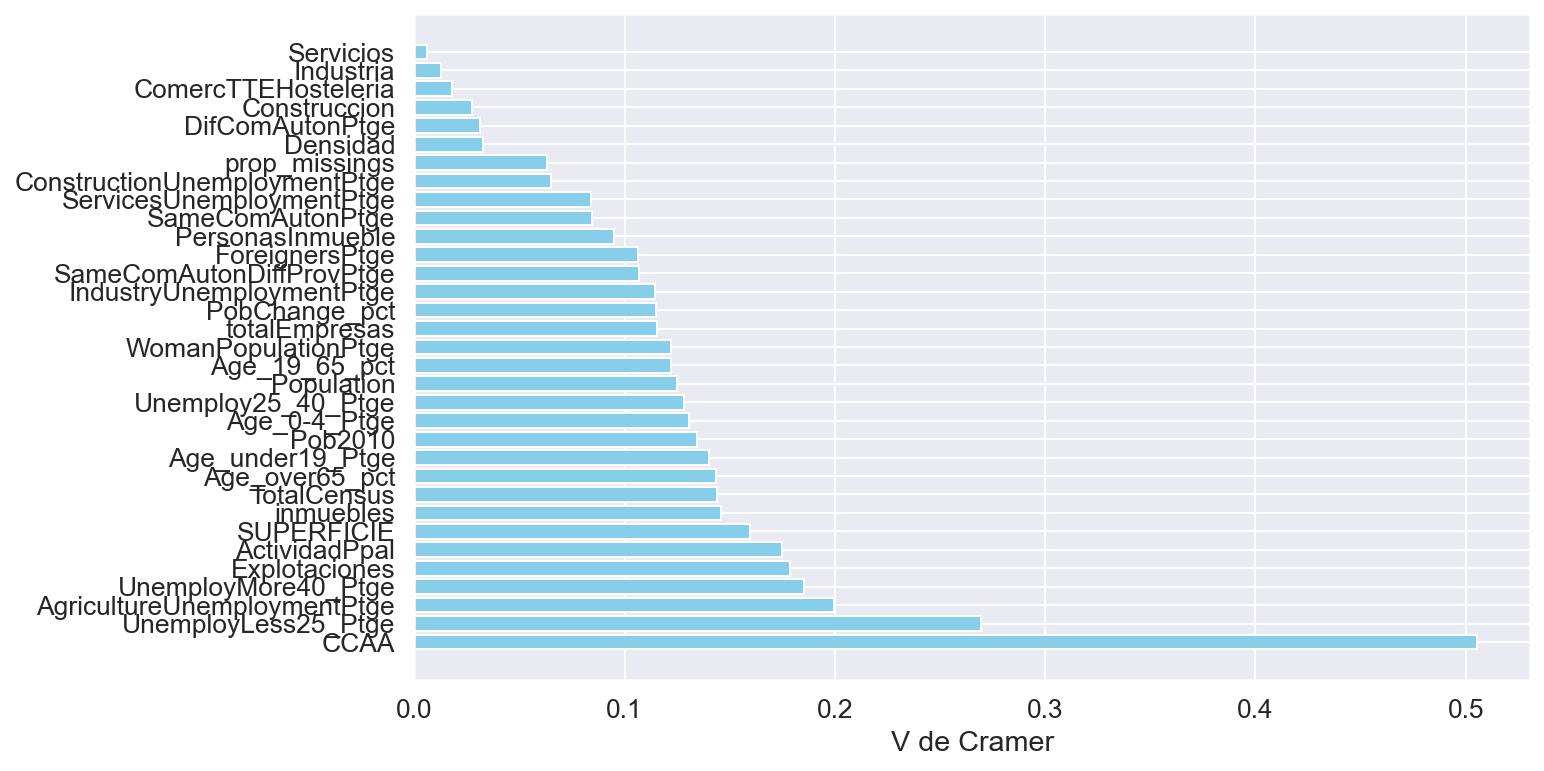
\includegraphics[width=\textwidth]{ejecuciones/vcramer_bin.png}
        \caption{V de Cramer para la variable binaria}
        \label{fig:cramerbin}
    \end{minipage}%
    \begin{minipage}{0.5\textwidth}
        \centering
        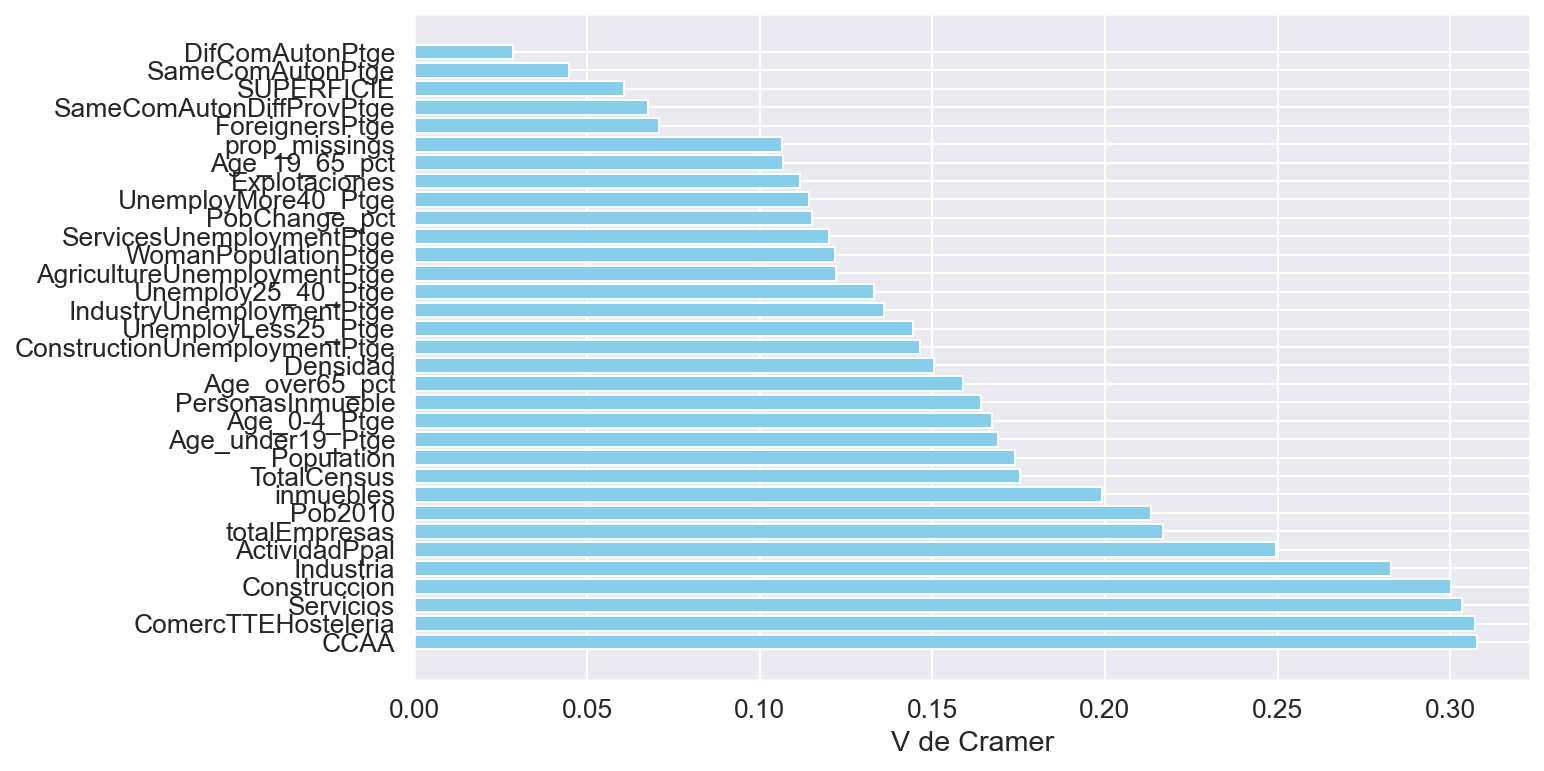
\includegraphics[width=\textwidth]{ejecuciones/vcramer_cont.png}
        \caption{V de Cramer para la variable continua}
        \label{fig:cramercont}
    \end{minipage}
\end{figure}

Como se ve, la variable que más relación tiene con ambas variables objetivo es la CCAA, mientras que hay un número considerable de ellas que tiene un valor de 
la V de Cramer inferior a 0.1, en caso de la binaria, o de 0.15, en caso de la continua. De momento, no realizaremos nada con las variables, pero estos dos 
gráficos nos servirán para, al momento de seleccionar las variables para ambas regresiones, ver cuáles debemos descartar o no.

Lo que sí haremos en este punto es dibujar la \hyperref[fig:fig:matCorr]{matriz de correlación} entre las variables continuas, para ver si hay alguna variable
que debamos eliminar. Lo primero que observamos es que tenemos numerosas variables con un valor de 1 en esta matriz, lo cual nos indica una correlación perfecta 
entre las mismas. Son, concretamente, las variables TotalEmpresas, Industria, Construccion, ComercTTEHosteleria, Servicios, Inmuebles y Pob2010. Esto se debe a 
que dichas variables se refieren al número de empresas de x tipo que hay en el municipio, por lo que es de esperar que estén relacionadas no sólo con TotalEmpresas, 
sino también entre sí. Además, como es de esperar, encontramos una alta relación entre Population y totalCensus, así como entre Age\_under19\_Ptge y 
Age\_0-4\_Pctge, y Age\_over65\_pct, que presenta una elevada correlación negativa con el resto de variables referidas a los porcentajes de edad. Todas estas 
variables no serán tenidas en cuenta a la hora de pasar las variables a los modelos y, además, serán eliminadas. Concretamente, eliminaremos Population, 
TotalEmpresas, Age\_under19\_Ptge y Age\_over65\_pct.

\begin{center}
    \begin{figure}[h!]
        \centering
        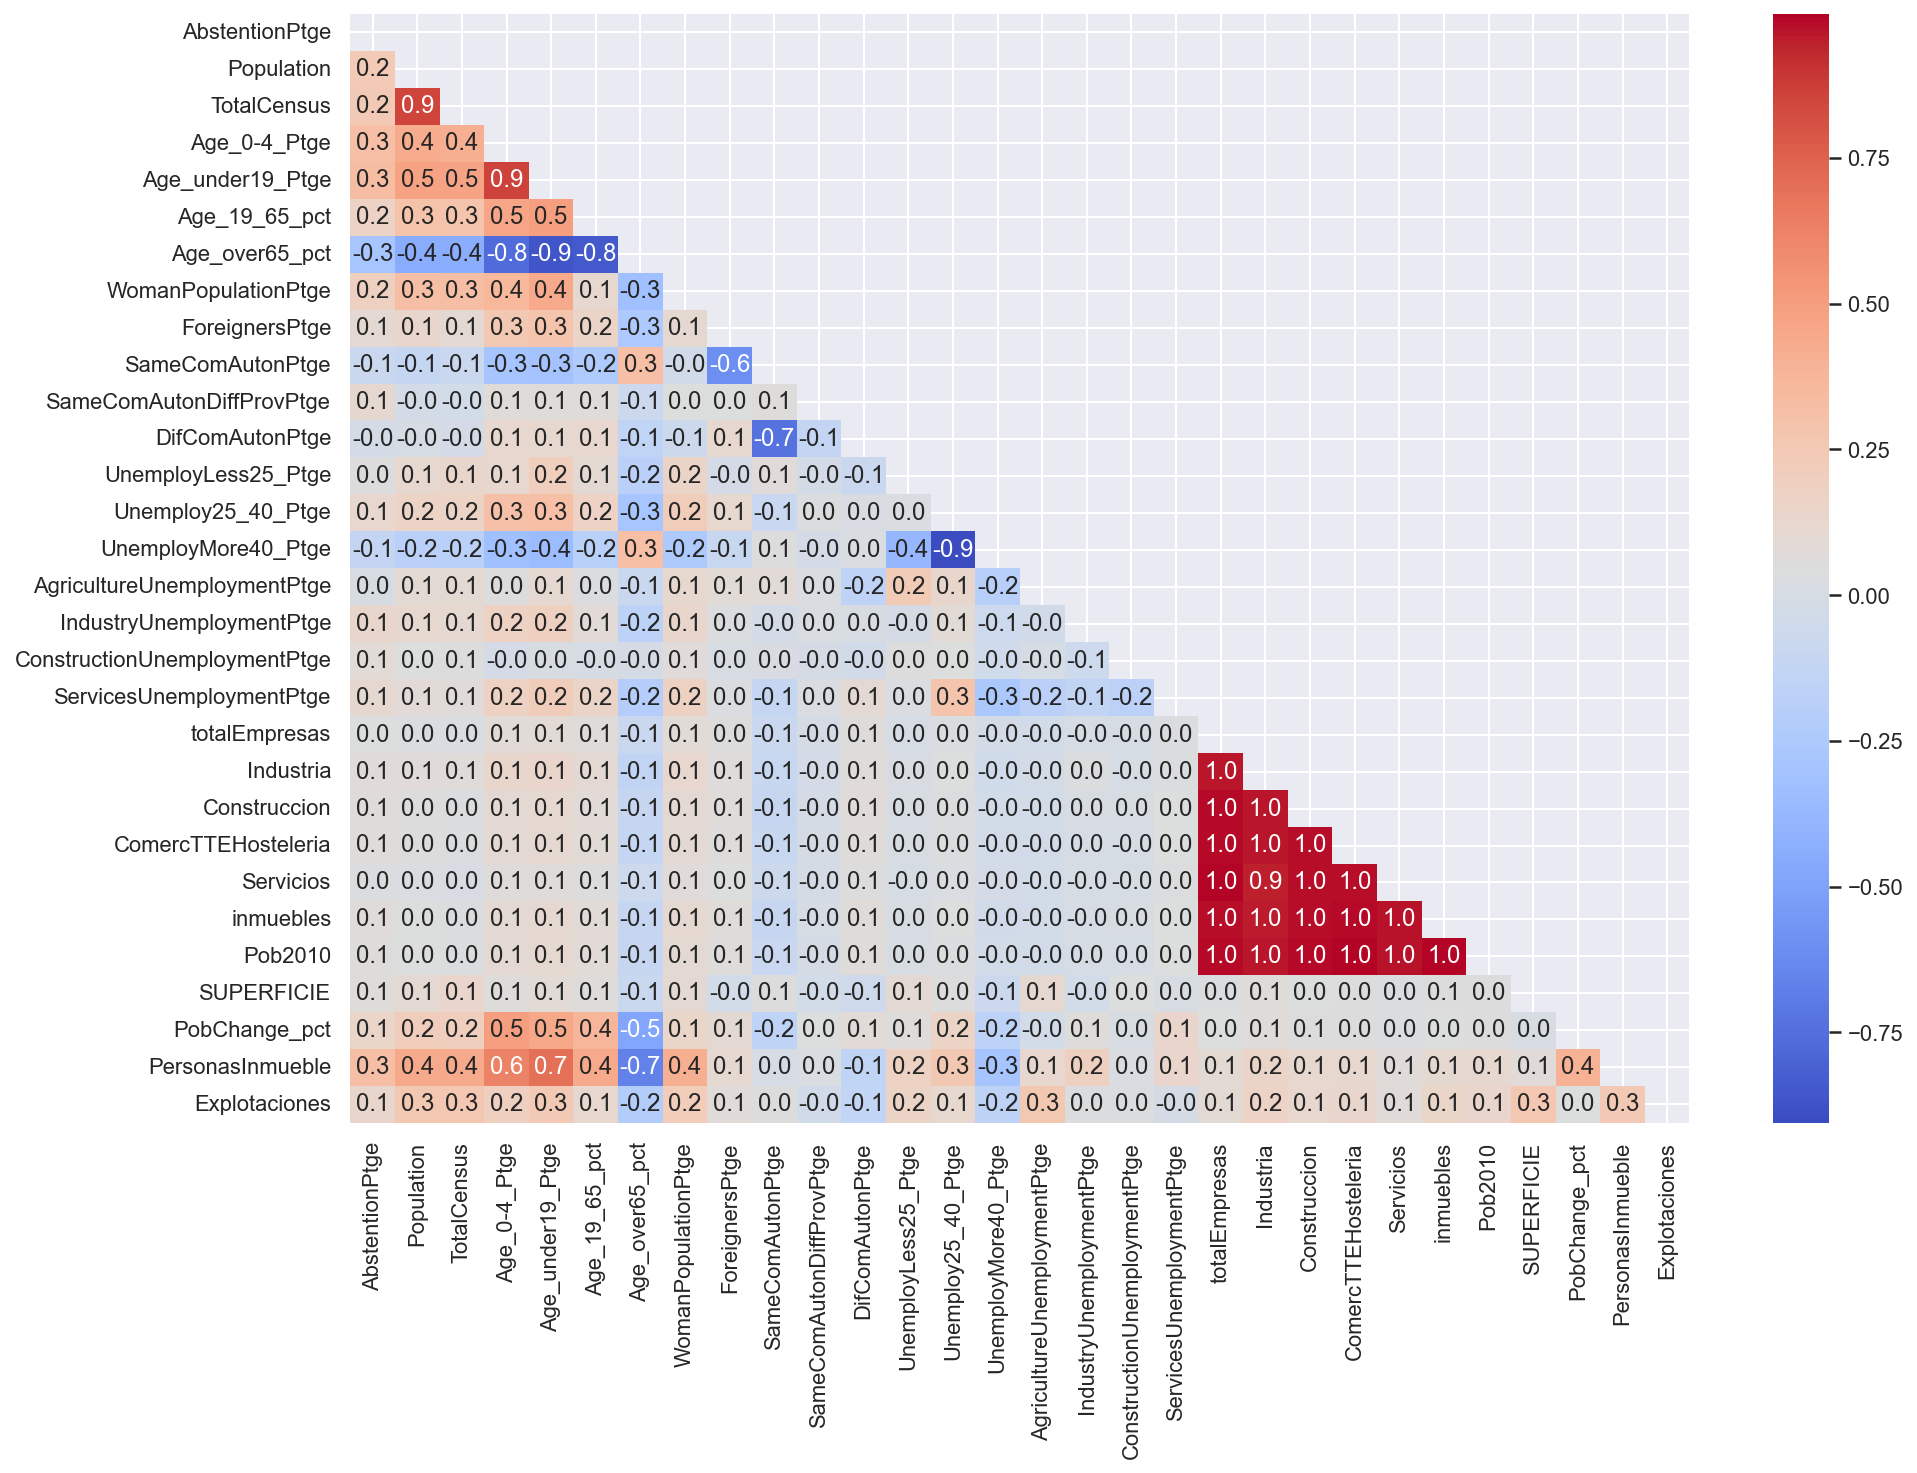
\includegraphics[width=0.7\textwidth]{ejecuciones/matCorr.png}
        \caption{Matriz de correlación de variables continuas}
        \label{fig:matCorr}
    \end{figure}
\end{center}

Una vez hemos realizado esto y eliminado estas variables para evitar que creen problemas de multicolinealidad, crearemos dos subconjuntos a partir de los datos:
\begin{lstlisting}[language=Python,numbers=none]
todo_cont = pd.concat([datos_input, varObjCont], axis = 1)
todo_bin = pd.concat([datos_input, varObjBin], axis = 1)
\end{lstlisting}
En uno de ellos, añadimos a los datos la variable objetivo continua, y al otro le añadimos la variable binaria. Estos serán los datos que empleemos para crear
los modelos de regresión.

\section{Regresión lineal}\label{lineal}
Antes de comenzar a realizar la selección de variables, debemos dividir los datos en un conjunto de entrenamiento y un conjunto de test, usando el 20\% de los 
datos como test (y el 80\% como entrenamiento).
\begin{lstlisting}[language=Python, numbers=none]
x_train, x_test, y_train, y_test = train_test_split(todo_cont, varObjCont, test_size = 0.2, random_state = 29112002)
\end{lstlisting}

\subsection{Selección clásica}\label{linclasica}
Debido a la capacidad computacional, a la correlación de variables estudiada en \ref{relaciones} y a los valores de la V de Cramer, es necesario descartar 
ciertas variables para la hora de crear el modelo. Como se explicó, se descartarán aquellas variables con correlación entre ellas, variables que puedan obtenerse
de otras (por ejemplo, TotalCensus se obtiene de Population), y las que tienen un valor de la V de Cramer más pequeño. De esta forma, las variables seleccionadas
son las siguientes:
\begin{lstlisting}[language=Python]
var_cont = ['TotalCensus', 'WomanPopulationPtge', 'UnemployLess25_Ptge', 'Unemploy25_40_Ptge', 'UnemployMore40_Ptge', 'AgricultureUnemploymentPtge', 'IndustryUnemploymentPtge', 'ConstructionUnemploymentPtge', 'ServicesUnemploymentPtge', 'PobChange_pct', 'PersonasInmueble', 'Explotaciones']
var_categ = ['CCAA', 'ActividadPpal', 'Densidad']
\end{lstlisting}

A continuación, se crean las interacciones entre las variables. Como se nos indica que únicamente debemos considerar las interacciones entre variables continuas,
la lista de interacciones será igual a la de variables continuas, pero podrían añadirse también las categóricas, lo cual probablemente daría también más robustez 
al modelo resultante. A partir de esta lista, se crea una lista con las interacciones únicas, dos a dos, de las variables. Esta será la que empleemos para la 
creación del modelo.
\begin{lstlisting}[language=Python]
interacciones = var_cont #+ var_categ
interacciones_unicas = list(itertools.combinations(interacciones, 2))
\end{lstlisting}

Una vez creadas las interacciones, emplearemos las funciones de lm para crear los modelos para la selección clásica de variables. En este caso, se crearán 6 
modelos: los resultantes de aplicar los métodos stepwise, backward y forward, empleando los criterios AIC y BIC. A modo de breve resumen, el método forward 
se caracteriza por crear un modelo añadiendo variables una a una, hasta que no haya ninguna variable que mejore el modelo; el backward comienza con todas 
las variables y va eliminando las menos significativas, hasta que solo queden aquellas significativas; y el stepwise es una combinación de los anteriores, 
iniciando con un modelo vacío y agregando variables más significativas, pero revisando tras cada adición si alguna variable ha dejado de serlo. Este es el que
proporciona un mejor equilibrio entre un modelo con muchas variables y uno que sea simple y eficiente. Respecto a los criterios AIC/BIC, el primero favorece 
modelos más complejos, mientras que el BIC penaliza más los modelos con más parámetros.
\begin{lstlisting}
modeloStepAIC = lm_stepwise(y_train, x_train, var_cont, var_categ, interacciones_unicas, 'AIC')
modeloBackAIC = lm_backward(y_train, x_train, var_cont, var_categ, interacciones_unicas, 'AIC')
modeloForwAIC = lm_forward(y_train, x_train, var_cont, var_categ, interacciones_unicas, 'AIC')
modeloStepBIC = lm_stepwise(y_train, x_train, var_cont, var_categ, interacciones_unicas, 'BIC')
modeloBackBIC = lm_backward(y_train, x_train, var_cont, var_categ, interacciones_unicas, 'BIC')
modeloForwBIC = lm_forward(y_train, x_train, var_cont, var_categ, interacciones_unicas, 'BIC')
\end{lstlisting}

Una vez hemos obtenido los 6 modelos, debemos elegir el ganador de entre ellos. Para ello, tenemos la tabla \ref{table:tablalineal}, que la hemos obtenido con
el código que se muestra a continuación (variando para cada modelo). En general, podemos observar unos valores de $R^2$ bastante bajos, lo que significa que
el modelo no logra tener una capacidad predictiva demasiado elevada. Esto podría deberse a varios motivos, como que algunas de las variables que hemos 
seleccionado no tengan especial relación con la variable objetivo, que se hayan excluido variables que sí son relevantes, o que la relación entre las 
variables no sea lineal, o incluso que se hayan cometido algunos errores en el proceso de limpieza de datos que lleven a la presencia de ruido en los mismos. 

\begin{lstlisting}[language=Python]
Rsq(modelo['Modelo'], y_train, modelo['X']) # R2 de train
x_test = crear_data_modelo(x_test,modelo['Variables']['cont'], modelo['Variables']['categ'], modelo['Variables']['inter'])
Rsq(modelo['Modelo'], y_test, x_test) # R2 de test
len(modelo['Modelo'].params) # Número de parámetros
\end{lstlisting}

Con los datos de los que disponemos, debemos elegir el modelo que equilibre mejor el ajuste ($R^2$ train), la generalización ($R^2$ test) y un menor número de 
parámetros, ya que un número elevado de los mismos podría dar lugar a un sobreajuste del modelo. Analizando únicamente el $R^2$, podríamos pensar que el mejor
modelo es el \textit{Backward AIC}, ya que tiene un $R^2$ de train más elevado. Sin embargo, vemos también que es el que presenta una mayor diferencia entre el $R^2$ 
de train y el $R^2$ de test, así como el mayor número de parámetros con diferencia. Por otra parte, los modelos de \textit{Stepwise} y \textit{Forward} con BIC 
son los que presentan un menor $R^2$ para los datos de test, con lo que, pese a ser los modelos más parsimoniosos, son los que peor capacidad explicativa 
tienen, por lo que se descartan. El resto de modelos (\textit{Backward BIC}, \textit{Stepwise AIC} y \textit{Forward AIC}) presentan tanto un $R^2$ de test 
como de train muy similares, con lo cual balancean bien el ajuste con la generalización. Por tanto, para discriminar entre ellos, se elije el que menor número 
de parámetros tiene, que en este caso es el \textbf{Backward BIC}, ya que mantendrá la mejor de las capacidades predictivas de todos los modelos analizados,
siendo a la vez fácilmente interpretable por el bajo número de variables y disminuyendo el riesgo de un sobreajuste.

\begin{table}[]
    \begin{center}
        \begin{tabular}{ |c|c|c|c|c| } 
        \hline
        \textbf{Método} & \textbf{Métrica} & \textbf{$R^{2}$ test} & \textbf{$R^{2}$ train} & \textbf{Nº parámetros} \\
        \hline 
        Backward & AIC & 0.392081 & 0.336811 & 56 \\ 
        Backward & BIC & 0.383429 & 0.335341 & 35 \\ 
        Stepwise & AIC & 0.382744 & 0.333387 & 39 \\ 
        Stepwise & BIC & 0.369415 & 0.324226 & 18 \\ 
        Forward & AIC & 0.382683 & 0.332820 & 40 \\ 
        Forward & BIC & 0.369415 & 0.324227 & 18 \\ 
        \hline
        \end{tabular}
        \caption{Comparación de modelos de regresión lineal}
        \label{table:tablalineal}
    \end{center}
\end{table}

\subsection{Selección aleatoria}\label{linaleatoria}
Por otra parte, se nos pide realizar una selección aleatoria de las variables. Esto implica generar varias submuestras de forma aleatoria, para realizar 
sobre ellas una selección de variables clásica y generar un resumen de los modelos que se han generado, de forma que se elegirán los modelos que hayan sido 
generados más veces, ya que son más estables y buenos candidatos a que se les aplique la validación cruzada.

Para la selección aleatoria, el código empleado es el que se muestra a continuación, en el que se realizan 20 iteraciones para generar los modelos. Se ha 
elegido el método stepwise, porque es el más completo, ya que combina las ventajas del método forward con las del backward, permitiendo ''replantearse'' si 
una variable debe entrar al modelo o no con cada iteración
\begin{lstlisting}[language=Python]
variables_seleccionadas = {'Formula': [],'Variables': []}

for x in range(20):
    print('---------------------------- iter: ' + str(x))
    
    # Dividir los datos de entrenamiento en conjuntos de entrenamiento y prueba.
    x_train2, x_test2, y_train2, y_test2 = train_test_split(x_train, y_train, test_size = 0.3, random_state = 29112002 + x)
    
    # Realizar la selección stepwise utilizando el criterio BIC en la submuestra.
    modelo = lm_stepwise(y_train2.astype(int), x_train2, var_cont, var_categ, interacciones_unicas, 'BIC')
    
    # Almacenar las variables seleccionadas y la fórmula correspondiente.
    variables_seleccionadas['Variables'].append(modelo['Variables'])
    variables_seleccionadas['Formula'].append(sorted(modelo['Modelo'].model.exog_names))
    
variables_seleccionadas['Formula'] = list(map(lambda x: '+'.join(x), variables_seleccionadas['Formula']))
\end{lstlisting}

Una vez generados los modelos, podemos calcular la frecuencia de cada fórmula, para con ello ver cuales son los dos modelos más frecuentes y sus 
correspondientes variables.

\begin{lstlisting}[language=Python]
frecuencias = Counter(variables_seleccionadas['Formula'])
frec_ordenada = pd.DataFrame(list(frecuencias.items()), columns = ['Formula', 'Frecuencia'])
frec_ordenada = frec_ordenada.sort_values('Frecuencia', ascending = False).reset_index()

# Identificar las dos modelos más frecuentes y las variables correspondientes.
var_1 = variables_seleccionadas['Variables'][variables_seleccionadas['Formula'].index(frec_ordenada['Formula'][0])]
var_2 = variables_seleccionadas['Variables'][variables_seleccionadas['Formula'].index(frec_ordenada['Formula'][1])]
\end{lstlisting}

De esta forma, podemos ver que las salidas de los modelos que más se repiten son las siguientes para el modelo 1 y el modelo 2:
\begin{lstlisting}[numbers=none]
{'cont': [],
 'categ': ['CCAA', 'ActividadPpal'],
 'inter': [('Unemploy25_40_Ptge', 'UnemployMore40_Ptge'),  ('ConstructionUnemploymentPtge', 'Explotaciones'),  ('ConstructionUnemploymentPtge', 'ServicesUnemploymentPtge'), ('UnemployLess25_Ptge', 'ServicesUnemploymentPtge'),  ('ConstructionUnemploymentPtge', 'PersonasInmueble'),  ('UnemployMore40_Ptge', 'IndustryUnemploymentPtge')]
}
\end{lstlisting}
\begin{lstlisting}[numbers=none]
{'cont': [],
'categ': ['CCAA', 'ActividadPpal'],
'inter': [('Unemploy25_40_Ptge', 'UnemployMore40_Ptge'), ('ConstructionUnemploymentPtge', 'Explotaciones'), ('UnemployLess25_Ptge', 'ServicesUnemploymentPtge'), ('ConstructionUnemploymentPtge', 'ServicesUnemploymentPtge'), ('Unemploy25_40_Ptge', 'ConstructionUnemploymentPtge'), ('UnemployMore40_Ptge', 'PersonasInmueble'), ('UnemployMore40_Ptge', 'IndustryUnemploymentPtge'), ('UnemployLess25_Ptge', 'PobChange_pct')]
}
\end{lstlisting}


\subsection{Modelo ganador}\label{linganador}
Una vez hemos determinado el modelo ganador de la \hyperref[linclasica]{selección clásica}, y obtenido los dos modelos que más se repiten en la 
\hyperref[linaleatoria]{selección aleatoria}, realizaremos la validación cruzada para determinar el modelo ganador de entre los tres. Para ello, se realizan 
50 ejecuciones de un bucle en el que aplicamos la función proporcionada \texttt{validacion\_cruzada\_lm} a los tres modelos, y mostramos los resultados en un 
boxplot para determinar el ganador.

\begin{lstlisting}[language=Python]
results = pd.DataFrame({'Rsquared': [], 'Resample': [], 'Modelo': []})

# Realizamos la validación cruzada
for rep in range(50):
    modelo1 = validacion_cruzada_lm(5, x_train, y_train, ganador['Variables']['cont']
                , ganador['Variables']['categ'], ganador['Variables']['inter'])
    modelo2 = validacion_cruzada_lm(5, x_train, y_train, var_1['cont'], var_1['categ'], var_1['inter'])
    modelo3 = validacion_cruzada_lm(5, x_train, y_train, var_2['cont'], var_2['categ'], var_2['inter'])
    
    results_rep = pd.DataFrame({
        'Rsquared': modelo1 + modelo2 + modelo3 
        , 'Resample': ['Rep' + str((rep + 1))]*5*3
        , 'Modelo': [1]*5 + [2]*5 + [3]*5 
    })
    results = pd.concat([results, results_rep], axis = 0)

# Dibujamos el boxplot
plt.figure(figsize=(10, 6))
plt.grid(True)
grupo_metrica = results.groupby('Modelo')['Rsquared']
boxplot_data = [grupo_metrica.get_group(grupo).tolist() for grupo in grupo_metrica.groups]
plt.boxplot(boxplot_data, labels=grupo_metrica.groups.keys()) 
plt.xlabel('Modelo')  
plt.ylabel('Rsquared') 
plt.show()  
\end{lstlisting}

\begin{center}
    \begin{figure}[h!]
        \centering
        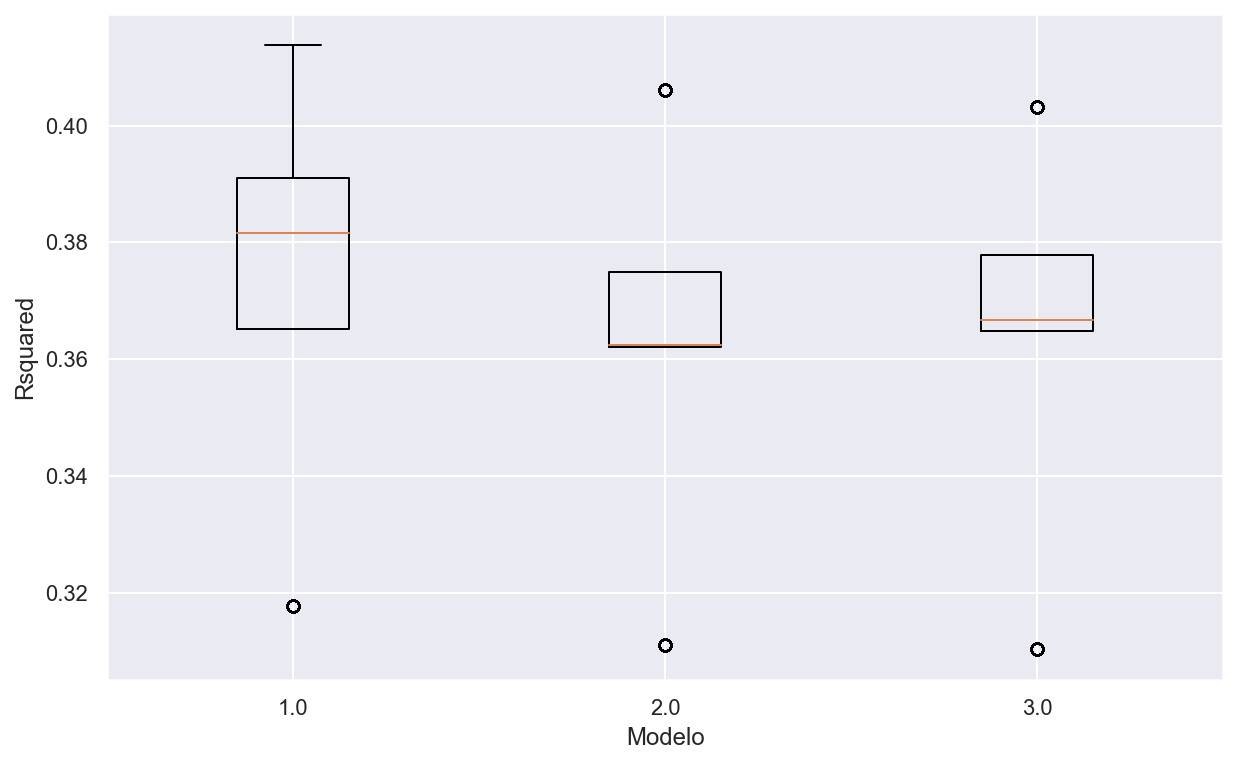
\includegraphics[width=0.6\textwidth]{ejecuciones/boxplot_lineal.png}
        \caption{Validación cruzada para regresión lineal}
        \label{fig:boxplotlin}
    \end{figure}
\end{center}

Como se puede ver en el boxplot, el claro ganador es el modelo 1, es decir, el que obtuvimos de la \hyperref[linclasica]{selección clásica}, ya que, aunque 
sí es cierto que presenta un variabilidad mayor, si observamos el número de parámetros vemos que es de 35 (\texttt{len(ganador[`Modelo`].params)}), mientras que
para los otros dos (\texttt{len(frec\_ordenada[`Formula`][0].split(`+`))} y \texttt{len(frec\_ordenada[`Formula`][1].split(`+`))}) es de 490 y 565, por lo que 
esta ligera mejora en la variabilidad no justifica en absoluto el aumento desmedido del número de parámetros.

\begin{center}
    \begin{figure}[h!]
        \centering
        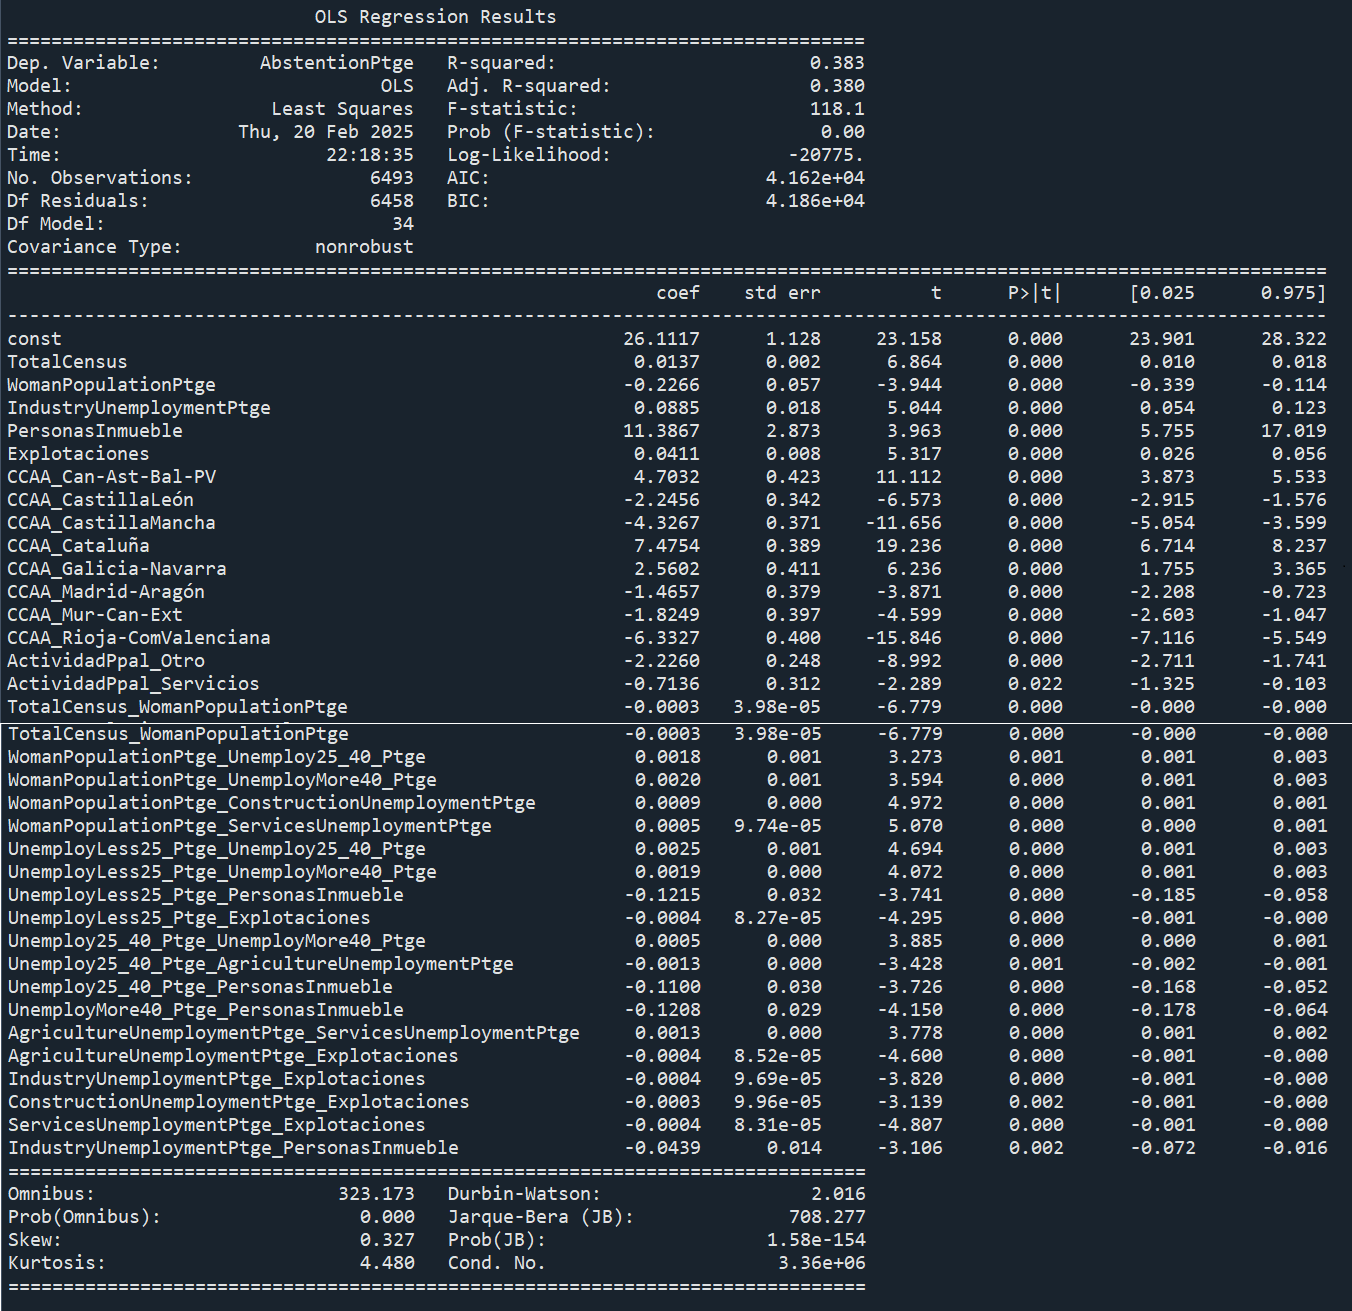
\includegraphics[width=0.7\textwidth]{ejecuciones/ganador_lineal.png}
        \caption{Resumen del modelo ganador de regresión lineal}
        \label{fig:summarylin}
    \end{figure}
\end{center}

Analizaremos algunos de los parámetros que nos devuelve el summary del modelo ganador con el objetivo de justificar por qué es el ganador. Como se indicó su 
$R^2$ para el conjunto de train es de 0.383, mientras que el $R^2$ ajustado es de 0.380, lo cual nos indica que aproximadamente el 38\% de variabilidad en el 
porcentaje de abstención se explica por las variables incluidas en el modelo. Es un porcentaje bajo, pero hay que tener en cuenta que datos como los de las 
elecciones son muy sensibles y dependen de muchos factores, incluso personales. Con 35 parámetros, tiene un buen equilibro entre capacidad explicativa y 
sencillez, evitando también el sobreajuste. Analizando la contribución de cada variable al $R^2$, vemos que la que más aporta (la que más influencia tiene) es 
la CCAA, con un $R^2$ de 0.211; mientras que las que tienen una aportación más marginal son, por ejemplo, IndustryUnemploymentPtge\_PersonasInmueble o 
ConstructionUnemploymentPtge\_Explotaciones, ambas con 0.0009.

Por otra parte, el summary nos devuelve los coeficientes para cada variable. Para la variable binaria CCAA\_Cataluña, tenemos un coeficiente de 7.4754 con un 
p < 0.01, lo cual indica que el resultado es altamente significativo. Esto significa que, en promedio, ser de Cataluña se asocia con un incremento aproximado
de 7.48 puntos porcentuales en la tasa de abstención respecto a otras CCAA, lo que nos indica que es una comunidad más abstencionista. Para la variable 
continua WomanPopulationPtge, tenemos un coeficiente de -0.2266 y un p < 0.01, lo que indica resultados altamente significativos. El coeficiente negativo indica 
que cada aumento de 1 punto porcentual en el porcentaje de mujeres de un municipio se asocia con una reducción de 0.23 puntos porcentuales en la tasa de 
abstención. Esto nos sugiere que allí donde hay más presencia femenina hay menor abstención, ya que las mujeres suelen estar mucho más movilizadas a la hora 
de votar.

En cuanto a su calidad, para evaluarla nos basamos en tres parámetros. Por una parte tenemos el estadístico de Durbin-Watson, que mide la autocorrelación de 
los residuos del modelo, con valores entre 0 y 4, donde valores próximos a 0 indican una autocorrelación positiva y valores cercanos a 4 una autocorrelación 
negativa, mientras que valores en torno a 2 indican que no presentan una autocorrelación significativa. Por otra parte, tenemos la prueba de Jarque-Bera, que 
evalúa si los residuos siguen una distribución normal empleando para ello la asimetría (si están equilibrados alrededor de la media) y la curtosis (si las colas 
son más aplanadas o no respecto a la normal). Un valor  de probabilidad bajo, menor que 0.05, implicaría que los residuos no siguen una distribución normal.
Por último, el número de condición, que mide la multicolinealidad del modelo, donde valores inferiores a 30 indican que no hay problemas de multicolinealidad, 
entre 30 y 100 una multicolinealidad moderada, y superiores a 100 indican que hay variables fuertemente correlacionadas.

Como podemos ver en la imagen \ref{fig:summarylin}, el valor de Durbin-Watson es de 2.016, lo que indica que no hay autocorrelación entre los residuos del modelo.
Sin embargo, el valor de la probabilidad de la prueba de Jarque-Bera es prácticamente nulo ($1*10^{-154}$), indicando que los residuos no siguen una distribución normal.
Sin embargo, esto puede que no genere problemas en una muestra tan grande como la nuestra, ya que según el Teorema del Límite Central, las variables se 
aproximarían a una distribución normal. Por último, el número de condición es extremadamente alto, de $3.36*10^6$, lo que sugiere una multicolinealidad fuerte.
Esto podría generar problemas en la predicción o dificultad para interpretar coeficientes. Podrían usarse técnicas para regularizar los coeficientes, o volver
a revisar las correlaciones, para corregir estos errores. En general, el modelo, si bien podría ser útil para realizar predicciones, no sirve mucho para 
interpretar las relaciones causales entre las variables, pero esto biene causado también por la naturaleza de los datos, ya que la abstención es un fenómeno 
que en general resulta difícil de predecir.

\section{Regresión logística}\label{logistica}
Respecto a la regresión logística, este apartado es muy similar al de la \hyperref[lineal]{regresión lineal}, por lo que aquí solo explicaremos los cambios 
más relevantes respecto al mismo.

Al igual que en dicho apartado, emplearemos la partición de datos en entrenamiento y test, renombrando las variables con un ''\_log'' para diferenciarlas. 
Además, en este caso, ya que tratamos con una variable dicotómica, comprobamos que efectivamente toma sólo dos valores, viendo que el valor 0 se registra un total de 6308 veces, y el 1 un total de 1809. No es una distribución simétrica,
pero sí que tomma los valores esperados, a fin de cuentas.
\begin{lstlisting}[language=Python, numbers=none]
pd.DataFrame({'n': varObjBin.value_counts(), '%': varObjBin.value_counts(normalize = True)})
\end{lstlisting}

\subsection{Selección clásica}\label{logclasica}
En este caso, igual que en la selección clásica para la lineal, se deben eliminar una serie de variables en base al valor de la V de Cramer que obtuvimos en
\ref{relaciones}, puesto que son variables poco significativas, y dado que la capacidad computacional de la que disponemos es limitada, debemos prescindir de 
ellas para poder generar los modelos en un tiempo razonable. Así, la lista de variables seleccionadas es la siguiente:
\begin{lstlisting}[language=Python]
var_cont_log = ['TotalCensus', 'WomanPopulationPtge', 'UnemployLess25_Ptge', 'Explotaciones', 'Unemploy25_40_Ptge', 'UnemployMore40_Ptge', 'AgricultureUnemploymentPtge']
var_categ_log = ['CCAA', 'ActividadPpal', 'Densidad']
\end{lstlisting}
Creamos también las interacciones entre las variables, aunque en este caso, claro, serán bastante más inferiores. Para generar los modelos, empleamos 
también funciones, pero en este caso las de glm, para generar los 6 modelos de la misma forma.
\begin{lstlisting}[language=Python]
modeloLogStepAIC = glm_stepwise(y_train_log, x_train_log, var_cont_log, var_categ_log, interacciones_unicas_log, 'AIC')
modeloLogStepBIC = glm_stepwise(y_train_log, x_train_log, var_cont_log, var_categ_log, interacciones_unicas_log, 'BIC')
modeloLogForwAIC = glm_forward(y_train_log, x_train_log, var_cont_log, var_categ_log, interacciones_unicas_log, 'AIC')
modeloLogForwBIC = glm_forward(y_train_log, x_train_log, var_cont_log, var_categ_log, interacciones_unicas_log, 'BIC')
modeloLogBackAIC = glm_backward(y_train_log, x_train_log, var_cont_log, var_categ_log, interacciones_unicas_log, 'AIC')
modeloLogBackBIC = glm_backward(y_train_log, x_train_log, var_cont_log, var_categ_log, interacciones_unicas_log, 'BIC')
\end{lstlisting}

Una vez generados los modelos, empleamos el siguiente código para crear la tabla con los valores del $R^2$ y del número de parámetros. Con este código,
obtenemos los valores de la tabla \ref{table:tablalogistica}.
\begin{lstlisting}[language=Python]
pseudoR2(modelo['Modelo'], modelo['X'], y_train_log)
x_test = crear_data_modelo(x_test_log,modelo['Variables']['cont'], modelo['Variables']['categ'], modelo['Variables']['inter'])
pseudoR2(modelo['Modelo'], x_test, y_test_log)
len(modelo['Modelo'].coef_[0])
\end{lstlisting}

\begin{table}[h!]
    \begin{center}
        \begin{tabular}{ |c|c|c|c|c| } 
        \hline
        \textbf{Método} & \textbf{Métrica} & \textbf{$R^{2}$ test} & \textbf{$R^{2}$ train} & \textbf{Nº parámetros} \\
        \hline 
        Backward & AIC & 0.269145 & 0.290712 & 15 \\ 
        Backward & BIC & 0.269145 & 0.290712 & 15 \\ 
        Stepwise & AIC & 0.270345 & 0.291749 & 15 \\ 
        Stepwise & BIC & 0.270345 & 0.291749 & 15 \\ 
        Forward & AIC & 0.271167 & 0.291983 & 19 \\ 
        Forward & BIC & 0.271167 & 0.291983 & 19 \\ 
        \hline
        \end{tabular}
        \caption{Comparación de modelos de regresión logística}
        \label{table:tablalogistica}
    \end{center}
\end{table}

En base a los parámetros obtenidos, lo primero que observamos es que aplicar la métrica AIC o BIC es completamente indiferente, ya que obtenemos los mismos 
resultados con una y con otra. Esto sugiere que los modelos tienen un buen balance entre ajuste y complejidad. También cabe destacar que el $R^2$ para train 
es siempre mayor que el de test, es decir, que generalizan mejor los datos nuevos. Para elegir el ganador, en primer lugar, descartamos el método backward, ya 
que es el que menor $R^2$ presenta (aunque cabe recalcar que la diferencia entre todos los $R^2$ es muy pequeña). Así, entre el método stepwise y el forward,
que presentan valores de $R^2$ de test y train prácticamente similares, elegiremos el modelo de Stepwise como el ganador, por presentar el menor número de 
parámetros. Entre el criterio AIC y el BIC, esta vez elegiremos el AIC, ya que puesto que emplean el mismo número de parámetros, minimiza la pérdida de 
información y nos da un enfoque más predictivo.

\subsection{Selección aleatoria}\label{logaleatoria}
Se nos pide igualmente hacer una selección aleatoria de variables, para lo cual se ha elegido también el método stepwise, como en el apartado \ref{linaleatoria},
por ser el más completo. Para ello, se emplea exactamente el mismo código que en dicho apartado, tanto para generar los modelos con selección aleatoria, como 
para calcular la frecuencia de cada fórmula. Si vemos las salidas de los modelos que se repiten, estas son:
\begin{lstlisting}[numbers=none]
{'cont': [],
'categ': ['CCAA'],
'inter': [('Explotaciones', 'UnemployMore40_Ptge'), ('TotalCensus', 'Unemploy25_40_Ptge'), ('TotalCensus', 'UnemployLess25_Ptge'), ('TotalCensus', 'AgricultureUnemploymentPtge')]
}
\end{lstlisting}
\begin{lstlisting}[numbers=none]
{'cont': [],
'categ': ['CCAA'],
'inter': [('Explotaciones', 'UnemployMore40_Ptge'), ('TotalCensus', 'UnemployLess25_Ptge'), ('TotalCensus', 'Unemploy25_40_Ptge'), ('WomanPopulationPtge', 'AgricultureUnemploymentPtge')]
}
\end{lstlisting}

\subsection{Modelo ganador}\label{logganador}
Una vez determinado el modelo ganador de la selección clásica, y con los dos de la selección aleatoria, realizaremos la validación cruzada para determinar el
modelo ganador. Para ello, se crean los tres modelos (resultantes del modelo ganador, y los dos de las variables elegidas mediante selección aleatoria),
y se definen para ellos el conjunto de test, mediante la función \texttt{crear\_data\_modelo}, y se crean los boxplot empleando el siguiente código:
\begin{lstlisting}[language=Python]
results_log = pd.DataFrame({'AUC': [], 'Resample': [], 'Modelo': []})
for rep in range(10):
    # Realiza validación cruzada en cuatro modelos diferentes y almacena sus R-squared en listas separadas
    modelo1VC = validacion_cruzada_glm(5, x_train_log, y_train_log, var_1_log['cont'], var_1_log['categ'], var_1_log['inter'])
    modelo2VC = validacion_cruzada_glm(5, x_train_log, y_train_log, var_2_log['cont'], var_2_log['categ'], var_2_log['inter'])
    modelo3VC = validacion_cruzada_glm(5, x_train_log, y_train_log, ganador_log['Variables']['cont'], ganador_log['Variables']['categ'], ganador_log['Variables']['inter'])
    
    # Crea un DataFrame con los resultados de validación cruzada para esta repetición
    results_rep = pd.DataFrame({
        'AUC': modelo1VC + modelo2VC + modelo3VC
        , 'Resample': ['Rep' + str((rep + 1))]*5*3  # Etiqueta de repetición (5 repeticiones 6 modelos)
        , 'Modelo': [1]*5 + [2]*5 + [3]*5  # Etiqueta de modelo (6 modelos 5 repeticiones)
    })
    results_log = pd.concat([results_log, results_rep], axis = 0)
\end{lstlisting}

Con ello, creamos el boxplot igual que hicimos antes, pero dibujando el Área bajo la curva ROC (esto es, cómo varía el rendimiento del modelo según se cambia
el punto de corte o umbral para predecir la variable objetivo, que en nuestro caso era que la suma de los votos de izquierda fuese mayor a los de derecha; un 
valor de 1 indica un rendimiento perfecto, e inferior a 0.5 indica que el modelo hace más prediciones incorrectas que buenas), y obtenemos el siguiente boxplot, 
donde determinamos que el modelo ganador es el segundo. Si vemos el AUC, vemos que es ligeramente superior a la del modelo 1, e igual a la del modelo 3, pero 
tiene menos desviación que el modelo3, por lo que se elige este modelo como ganador.
\begin{center}
    \begin{figure}[h]
        \centering
        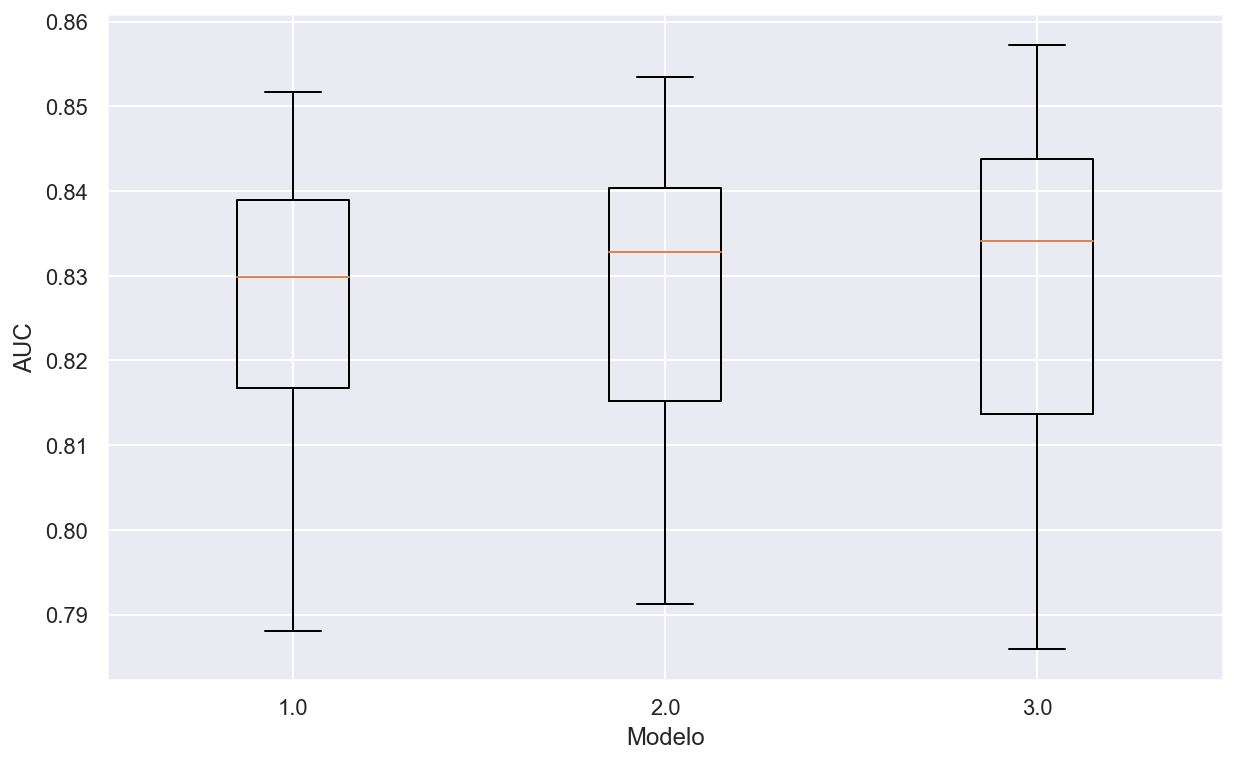
\includegraphics[width=0.6\textwidth]{ejecuciones/boxplot_logistica.png}
        \caption{Validación cruzada para regresión logística}
        \label{fig:boxplotlog}
    \end{figure}
\end{center}

A continuación empleamos el siguiente código para encontrar los puntos de corte, los cuales mostramos en el plot \ref{fig:puntoscorte}. Estos puntos de corte,
como comentamos, definen la probabilidad a partir de la cual se considera que un caso pertenece a la clase positiva (es decir, un municipio mayoritariamente de
izquierdas). Por una parte, el índice de Youden, que prioriza la sensibilidad (detectar la mayoría de casos positivos) es de 0.23, mientras que el de Accuracy 
(maximizando la precisión global del modelo) es de 0.5. Ya que, como analizamos en \ref{logistica}, el conjunto de datos estaba desbalanceado (había más valores 
para el 0 que para el 1), elegiremos el punto de corte basado en Youden, ya que es la mejor opción en un conjunto desbalanceado porque garantiza que el modelo
detecte ambos valores o clases de forma razonable, balanceando la sensibilidad con la especifidad. 
\begin{lstlisting}[language=Python]
posiblesCortes = np.arange(0, 1.01, 0.01).tolist()  # Generamos puntos de corte de 0 a 1 con intervalo de 0.01
rejilla = pd.DataFrame({'PtoCorte': [], 'Accuracy': [], 'Sensitivity': [], 'Specificity': [], 'PosPredValue': [], 'NegPredValue': []})
for pto_corte in posiblesCortes:  # Iteramos sobre los puntos de corte
    rejilla = pd.concat(
        [rejilla, sensEspCorte(modelo2['Modelo'], x_test_log, y_test_log, pto_corte, modelo2['Variables']['cont'], modelo2['Variables']['categ'], modelo2['Variables']['inter'])],
        axis=0
    )  # Calculamos las métricas para el punto de corte actual y lo agregamos al DataFrame

rejilla['Youden'] = rejilla['Sensitivity'] + rejilla['Specificity'] - 1  # Calculamos el índice de Youden
rejilla.index = list(range(len(rejilla)))  # Reindexamos el DataFrame para que los índices sean consecutivos    
\end{lstlisting}
\begin{figure}[h!]
    \centering
    \begin{minipage}{0.5\textwidth}
        \centering
        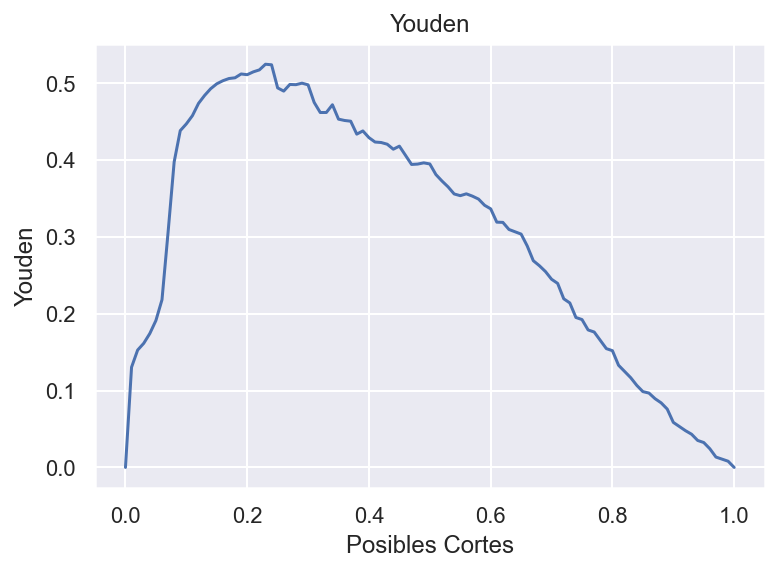
\includegraphics[width=\textwidth]{ejecuciones/cortesY.png}
    \end{minipage}%
    \begin{minipage}{0.5\textwidth}
        \centering
        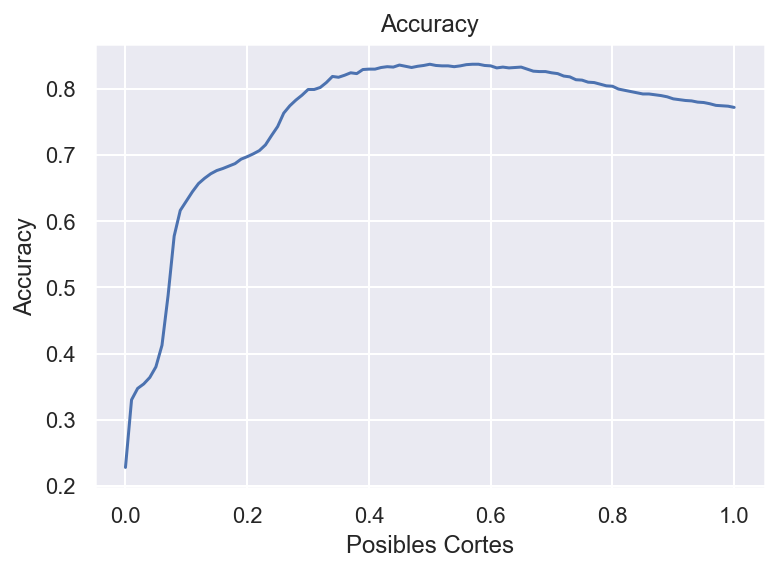
\includegraphics[width=\textwidth]{ejecuciones/cortesA.png}
    \end{minipage}
    \caption{Puntos de corte para Youden y Accuracy}
    \label{fig:puntoscorte}
\end{figure}

Una vez decidido el modelo ganador, vemos las variables más importantes del mismo, las que más aportan. En este caso, vemos que claramente la más importante es 
la CCAA, es decir, que podríamos decir que hay comunidades más de izquierdas que de derechas (algo que se suele ver en los resultados en general de las elecciones),
seguido de las interacciones entre TotalCensus y UnemployLess25\_Ptge y Unemploy25\_40\_Ptge, pero con muy poca aportación.
\begin{center}
    \begin{figure}[h]
        \centering
        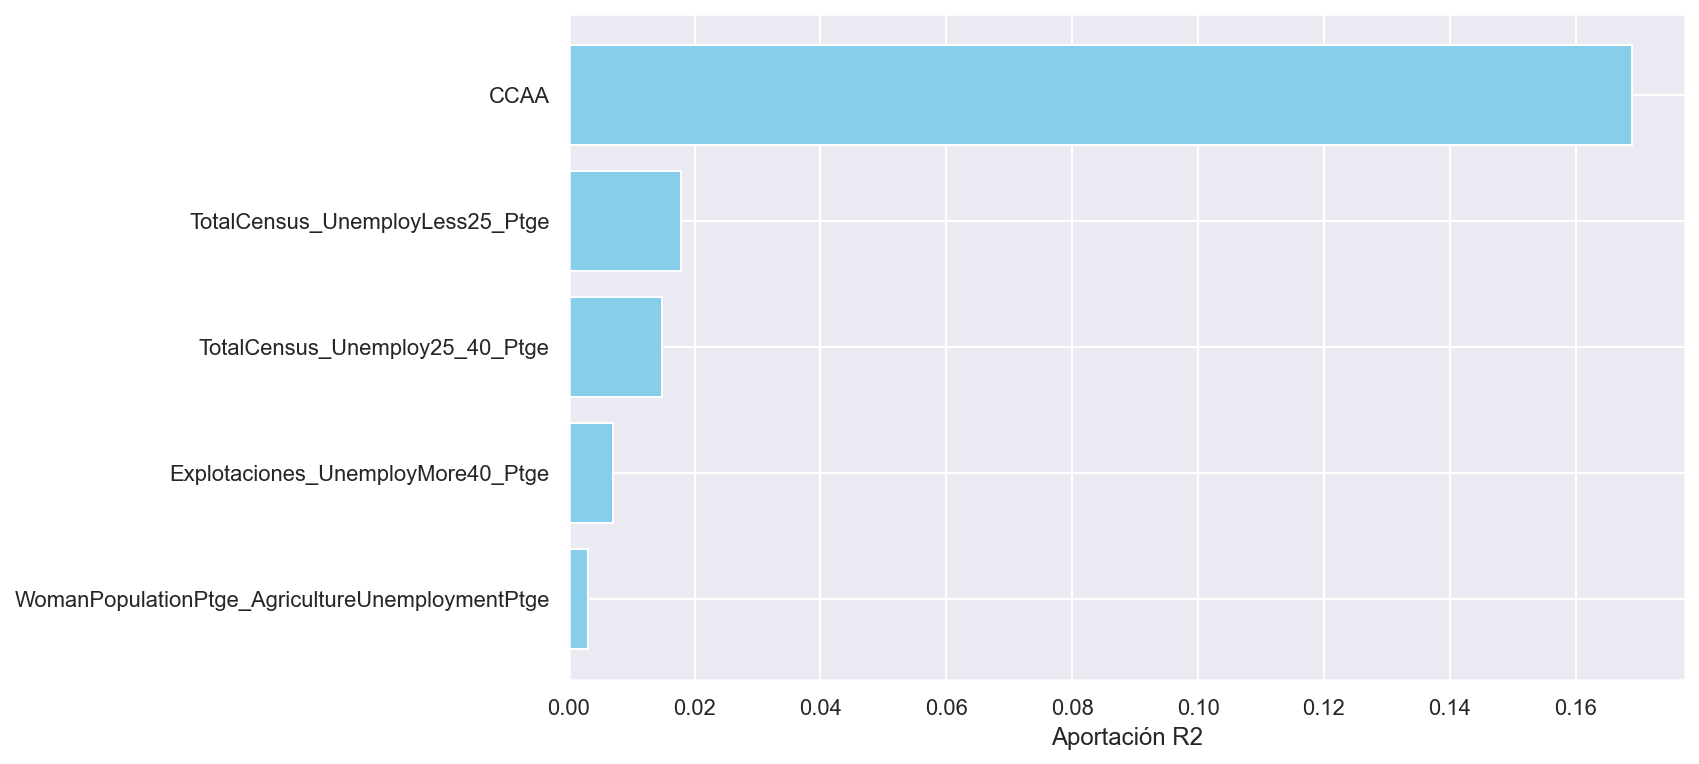
\includegraphics[width=0.75\textwidth]{ejecuciones/variables_log.png}
        \caption{Variables más importantes del modelo}
        \label{fig:variables}
    \end{figure}
\end{center}

Analizamos también la diferencia en el área bajo la curva para train y test (imagen \ref{fig:ROC}), donde vemos una curva bastante similar en ambos casos, y que 
se encuentra a medio camino entre la línea punteada azul (que representaría un área de 0.5) y el área completa.

\begin{figure}[h!]
    \centering
    \begin{minipage}{0.45\textwidth}
        \centering
        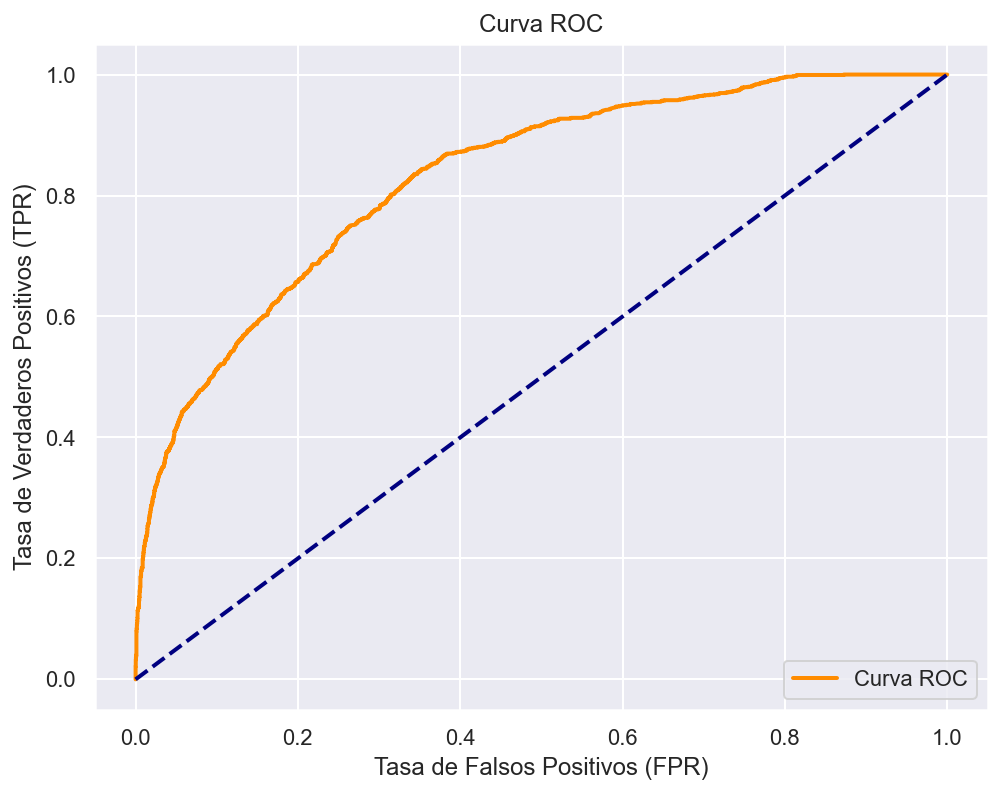
\includegraphics[width=\textwidth]{ejecuciones/ROC_train.png}
    \end{minipage}%
    \begin{minipage}{0.45\textwidth}
        \centering
        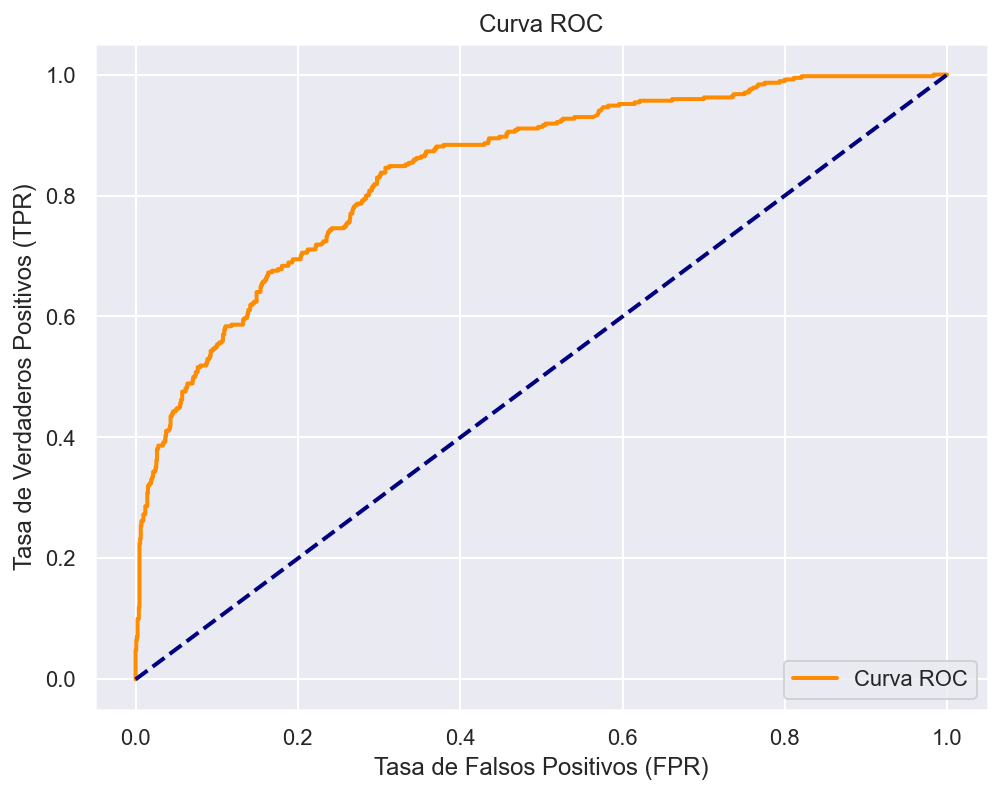
\includegraphics[width=\textwidth]{ejecuciones/ROC_test.png}
    \end{minipage}
    \caption{Área bajo la curva para train (izq.) y test (der.)}
    \label{fig:ROC}
\end{figure}

Por último, sólo queda analizar los coeficientes de dos variables y medir la calidad. La variable CCAA\_Cataluña tiene un coeficiente de -5.2996, el más 
negativo de todos. Esto quiere decir que los municipios que pertenecen a esta CCAA tienen menos posibilidades de que la Izquierda sea mayoritaria. Además, con 
un p-valor de 0, nos indica que el efecto es estadísticamente significativo. Por otra parte, la variable TotalCensus\_UnemployLess25\_Ptge tieneun coeficiente 
de 0.000067, positivo, lo que indica que conforme aumenta el porcentaje de desempleados menores de 25 en el censo total, aumenta la probabilidad de que el 
municipio sea de izquierdas. Con un p-valor de 0 también, es un efecto significativo, aunque el coeficiente tan pequeño indica que el impacto es bastante 
marginal en comparación con otras variables.

\begin{center}
    \begin{figure}[h]
        \centering
        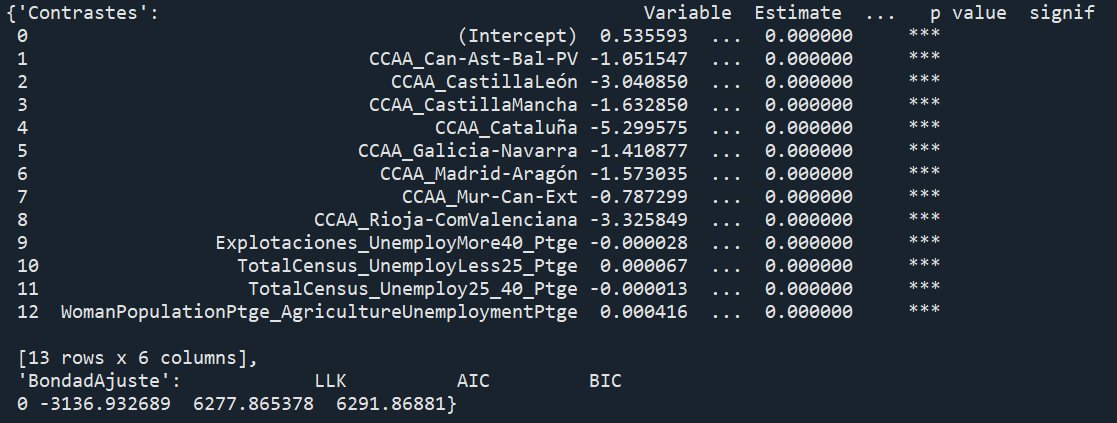
\includegraphics[width=0.75\textwidth]{ejecuciones/ganado_logistica.png}
        \caption{Resumen del modelo ganador de regresión logística}
        \label{fig:summarylog}
    \end{figure}
\end{center}

Sólo nos resta analizar la calidad, con la función \texttt{summary\_glm}, cuya ejecución se ve en la imagen \ref{fig:summarylog}. Obtenemos un AIC de $6277.87$, un BIC de 
$6291.87$ y un LLK de $-3136.93$. El LLK, o Log-Likelihood, mide qué tan bien los valores que predice el modelo explican los datos observados. Valores altos 
indican mejor ajuste, y valores negativos indican que el modelo no detecta bien los patrones en los datos. En este caso, el LLK sugiere un ajuste que no es 
óptimo, pero que podríamos considerar como moderado. Sin embargo, los valores de AIC y BIC tan elevados, lo que nos indica que podría estar sobreajustado o 
contener variables poco relevantes. Sería interesante poder probar otras técnicas de selección de variables para poder optimizar el modelo, pero sin dejar 
de tener en cuenta que estamos intentando predecir variables que dependen de muchos más factores a parte de aquellos que se nos han dado, por lo que son 
difíciles de predecir.

\end{sloppypar}
\end{document}
